\documentclass[11pt,a4paper,twoside]{tesis}
% SI NO PENSAS IMPRIMIRLO EN FORMATO LIBRO PODES USAR
%\documentclass[11pt,a4paper]{tesis}

\usepackage{graphicx}
\usepackage[utf8]{inputenc}
\usepackage[spanish]{babel}
\usepackage[left=3cm,right=3cm,bottom=3.5cm,top=3.5cm]{geometry}
\usepackage{tipa}
\usepackage{booktabs}

\usepackage{floatrow}
\floatplacement{figure}{H}
\floatplacement{table}{H}
\begin{document}
%%%% CARATULA

\def\autor{Franco Negri}
\def\tituloTesis{Implementación y evaluación de un sistema de sintesis de habla con acento extranjero variable}
\def\runtitle{Implementacíón y evaluación de un sistema de sintesis de habla}
%\def\runtitle{Star Wars: Rebellion and Empire}
\def\director{Agustin Gravano}
\def\codirector{Master Yoda}
\def\lugar{Buenos Aires, 2018}
\newcommand{\HRule}{\rule{\linewidth}{0.2mm}}
%
\thispagestyle{empty}

\begin{center}\leavevmode

\vspace{-2cm}

\begin{tabular}{l}

\includegraphics[width=2.6cm]{logofcen.pdf}
\end{tabular}


{\large \sc Universidad de Buenos Aires

Facultad de Ciencias Exactas y Naturales

Departamento de Computaci\'on}

\vspace{6.0cm}

%\vspace{3.0cm}
%{
%\Large \color{red}
%\begin{tabular}{|p{2cm}cp{2cm}|}
%\hline
%& Pre-Final Version: \today &\\
%\hline
%\end{tabular}
%}
%\vspace{2.5cm}

\begin{huge}
\textbf{\tituloTesis}
\end{huge}

\vspace{2cm}

{\large Tesis de Licenciatura en Ciencias de la Computaci\'on}

\vspace{2cm}

{\Large \autor}

\end{center}

\vfill

{\large

{Director: \director}

\vspace{.2cm}

%{Codirector: \codirector}

\vspace{.2cm}

\lugar
}

\newpage\thispagestyle{empty}


%%%% ABSTRACTS, AGRADECIMIENTOS Y DEDICATORIA
\frontmatter

%Intro
\pagestyle{empty}
%%\begin{center}
%\large \bf \runtitulo
%\end{center}
%\vspace{1cm}
\chapter*{\runtitulo}

\noindent La princesa Leia, líder del movimiento rebelde que desea reinstaurar la República en la galaxia en los tiempos ominosos del Imperio, es capturada por las malévolas Fuerzas Imperiales, capitaneadas por el implacable Darth Vader. El intrépido Luke Skywalker, ayudado por Han Solo, capitán de la nave espacial ``El Halcón Milenario'', y los androides, R2D2 y C3PO, serán los encargados de luchar contra el enemigo y rescatar a la princesa para volver a instaurar la justicia en el seno de la Galaxia (aprox. 200 palabras).

\bigskip

\noindent\textbf{Palabras claves:} Guerra, Rebelión, Wookie, Jedi, Fuerza, Imperio (no menos de 5).
%\cleardoublepage
%\begin{center}
%\large \bf \runtitle
%\end{center}
%\vspace{1cm}
\chapter*{\runtitle}

El presente trabajo tiene como objetivo generar un sistema de síntesis de habla en castellano con acento inglés. Si bien actualmente los métodos más avanzados para generar habla utilizan técnicas de aprendizaje automático basados en redes neuronales, en este trabajo utilizamos técnicas basadas en HMM+GMM por su practicidad. Utilizando esta técnica construimos modelos en castellano y en inglés y luego, interpolando sus características acústicas, intentamos producir un modelo capaz de sintetizar habla que resulte inteligible pero que contenga características atribuibles a un extranjero angloparlante hablando castellano. Para este trabajo la interpolación de características acústicas ocurre a nivel de fono, por lo que, para realizar la mezcla de modelos es necesario compatibilizar los fonos de ambos idiomas. Por este motivo, parte del trabajo consiste en desarrollar un mapeo entre los repertorios fonéticos del inglés y el castellano que resulte natural. Por último evaluamos el nivel de efectividad de nuestro método de manera experimental. Para ello desarrollamos una metodología de evaluación que nos permita medir tanto la ininteligibilidad de un audio, como el origen atribuido por los participantes.

Los resultados muestran con claridad que, como esperábamos, al aumentar el porcentaje de interpolación de inglés con castellano, aumenta la percepción de acento anglosajón en el habla sintetizada, al mismo tiempo que se deteriora su inteligibilidad.

\bigskip

\noindent\textbf{Keywords:} Síntesis de habla, HMM, HTS, GMM, acento extranjero, aprendizaje automático. % OPCIONAL: comentar si no se quiere
\cleardoublepage
\chapter*{Agradecimientos}

\noindent Lorem ipsum dolor sit amet, consectetur adipiscing elit. Fusce sapien ipsum, aliquet eget convallis at, adipiscing non odio. Donec porttitor tincidunt cursus. In tellus dui, varius sed scelerisque faucibus, sagittis non magna. Vestibulum ante ipsum primis in faucibus orci luctus et ultrices posuere cubilia Curae; Mauris et luctus justo. Class aptent taciti sociosqu ad litora torquent per conubia nostra, per inceptos himenaeos. Mauris sit amet purus massa, sed sodales justo. Mauris id mi sed orci porttitor dictum. Donec vitae mi non leo consectetur tempus vel et sapien. Curabitur enim quam, sollicitudin id iaculis id, congue euismod diam. Sed in eros nec urna lacinia porttitor ut vitae nulla. Ut mattis, erat et laoreet feugiat, lacus urna hendrerit nisi, at tincidunt dui justo at felis. Class aptent taciti sociosqu ad litora torquent per conubia nostra, per inceptos himenaeos. Ut iaculis euismod magna et consequat. Mauris eu augue in ipsum elementum dictum. Sed accumsan, velit vel vehicula dignissim, nibh tellus consequat metus, vel fringilla neque dolor in dolor. Aliquam ac justo ut lectus iaculis pharetra vitae sed turpis. Aliquam pulvinar lorem vel ipsum auctor et hendrerit nisl molestie. Donec id felis nec ante placerat vehicula. Sed lacus risus, aliquet vel facilisis eu, placerat vitae augue.
 % OPCIONAL: comentar si no se quiere
\cleardoublepage
\hfill \textit{A Agustin Gravano: Por tolerar mis faltas de ortografía}
  % OPCIONAL: comentar si no se quiere

\cleardoublepage
\tableofcontents

\mainmatter
\pagestyle{headings}

%%%% ACA VA EL CONTENIDO DE LA TESIS
%\section{Introducción}
%
\noindent Un sistema de Text To Speech (TTS) es aquel que genera habla artificial a partir de un texto de entrada. En la actualidad estos sistemas se encuentran incluidos en muchas aplicaciones domesticas, desde navegación por GPS, asistentes personales inteligentes (como es el caso de SIRI), ayuda para personas no videntes, traducción automática, etc.

\noindent En las últimas décadas se han visto grandes progresos en este campo, siendo capaces de modelar con cierto grado de efectividad cuestiones tales como la prosodia del hablante, emociones, etc. Si bien actualmente se considera que el estado del arte para la síntesis es el entrenamiento con redes neuronales profundas (DNN), una técnica todavía utilizada es la que utiliza modelos ocultos de markov mas modelos de mezcla de gaussianas (HMM+GMM) que, a partir de un corpus de datos de entrenamiento, extrae información acústica y genera un modelo probabilístico que permita sintetizar habla. 

Consideramos que este método si bien no nos permitirá obtener la mejor voz posible, nos permitirá entender mejor los features con los que trabajamos y por lo tanto modificarlos según consideremos conveniente, algo que puede volverse mas complicado cuando se esta trabajando con redes neuronales profundas.

\noindent En este trabajo de tesis se estudia una manera posible de generar un TTS basado en HMMs capaz de sintetizar habla en español con acento extranjero. Las razones por las que podría querer diseñarse un sistema con estas características varían desde un punto de vista puramente técnico, ya que un sistema así permitiría la utilización de corpus de entrenamiento de hablantes no nativos para la generación de una nueva voz, pasando por cuestiones lingüísticas, como es poder vislumbrar el limite en que un acento deja de parecernos local para pasar a ser extranjero y cuestiones psicológicas: lograr distintos efectos sobre el usuario, quien podría reaccionar distinto ante diferentes acentos.

\noindent En el transcurso de este trabajo se espera además evaluar la prosodia y la fonética del modelo generado con estas características, como así también evaluar su inteligibilidad. Además pretenderemos evaluar la efectividad de técnicas de speaker adaptation cuando se utilizan corpus de distintas nacionalidades con repertorios fonéticos disimiles (para este caso de estudio: castellano e ingles)

\noindent Para este trabajo nos basaremos fuertemente en la síntesis/análisis mel-cepstral, speech parameter modeling usando HMMs y speech parameter generation usando HMMs, como es descripto en la disertación doctoral \textit{Simultaneous Modeling of phonetic and prosodic parameters, and characteristic conversion for hmm-based text-to-speech systems} del Profesor Tadashi Kitamura, Nagoya Institute of Technology\cite{phoneticAndProsodic}.


Como introducción a este trabajo comenzaremos analizando las decisiones de metodología utilizadas a lo largo de la investigación, así también como detalles teóricos como el mapeo de fonemas necesario para adaptar el repertorio fonético del ingles al castellano, etc.

En las siguiente secciones se detallaran distintos temas que fueron necesarios abordar para llevar a cabo esta tesis. En orden de aparición estos son:

\begin{enumerate}
\item Realizar un etiquetado fonético de distintos corpus de audios.

\item Realizar un mapeo entre los fonos del castellano y los del ingles. Estos serán necesarios en el paso siguiente donde será requerimiento indispensable tener modelados los mismos fonos para todos los modelos.

\item Realizar el entrenamiento de los HMM+GMM. Para esto contaremos con el framework de modelado de HMMs HTS. 

\item Utilizar las herramientas provistas por HTS para interpolar entre modelos y poder sintetizar habla con distintos grados de fonética y prosodia inglesa.

\end{enumerate}

Para finalizar el apartado teórico discutiremos algunos aspectos implémentatelos de HTS y las otras herramientas utilizadas en este trabajo.

%\pagebreak
%Teoria
%Metodología
El objetivo de esta sección es dar una introducción a los corpus utilizados, junto con la teoría referente a las metodologías utilizadas para su procesamiento. Los detalles implementativos serán descriptos más adelante en la Sección \ref{herramientas}.

\subsection{Primer corpus en castellano}

Al inicio de la investigación, comenzamos con el corpus \textit{SECYT-mujer}, construido por el Laboratorio de Investigaciones Sensoriales (INIGEM, UBA-CONICET) \cite{secytMujer}. El mismo está compuesto por $741$ oraciones cortas declarativas habladas por una locutora profesional en castellano rioplatense, equivalentes a $48$ minutos de habla. A continuación, tres ejemplos de las oraciones articuladas por la locutora:

\indent\indent \textit{La voluntad del juez fue impuesta en tribunales.}

\indent\indent \textit{Los vinos uruguayos han mejorado en el último lustro.}

\indent\indent \textit{Al atardecer se puso su disfraz juglaresco.}

Como parte inicial del trabajo es indispensable construir el etiquetado fonético para el corpus. Estos etiquetados consistirán en una lista de fonos donde se indica cuándo comienza y termina cada uno en el audio. La calidad de las oraciones que logremos sintetizar a posteriori dependerá fuertemente del etiquetado, por lo que es necesario prestar especial cuidado en que las transcripciones estén lo mejor alineadamente posible con los audios. Las transcripciones serán necesarias para entrenar los modelos de HMM+GMM, extrayendo tanto la información acústica para cada fono (cosas tales como la frecuencia principal, la duración, etc), como así también información contextual (por ejemplo: cómo suena un fono cuando está seguido de algún otro, al principio de una oración, si se encuentra en un diptongo, etc). Por ende, una mala transcripción se traducirá indefectiblemente en un mal modelo y malas oraciones sintetizadas. Llevamos a cabo varias pruebas de concepto utilizando HTS en este corpus, experimentando con diversos métodos para obtener el etiquetado fonético. 

La primera estrategia consistió en utilizar alineamiento automático con \textit{EHMM alignment} \cite{phoneticCapturing} empleando Festival y Festvox. Esta técnica tienen como principal ventaja su sencillez. Para generar las transcripciones solo es necesario contar con el corpus que se quiere anotar y sus \textit{transcripciones grafémicas} (Transcripciones gráficas, escritas).

Los resultados preliminares con este método fueron bastante negativos: los audios generados resultaban poco inteligibles notándose claros defectos acústicos, el más notable siendo el fono /\textipa{r}/ (perro) que se asemejaba más a /\textipa{R}/ (pero).

Utilizando la herramienta de visualización y manipulación de audio Praat \cite{praat} para visualizar el alineamiento entre las transcripciones fonéticas y los audios, descubrimos que la alineación de algunas oraciones estaba desfasada algunas milésimas de segundo respecto de los audios. Dado que para el alineamiento automático es necesario alinear los audios del corpus con audios sintetizados con festival, sospechamos que pudo haber problemas con la calidad del corpus o que los audio sintetizados por Festival eran demasiado disimiles comparados con los audios reales. 

Dado que para el corpus contamos con las transcripciones fonéticas anotadas de manera manual, procedimos a implementar un híbrido, que consiste en tomar los tiempos de las anotaciones fonéticas manuales y la información contextual y el repertorio fonético generado a partir del proceso de EHMM y combinarlos en una nueva transcripción fonética. De esta manera buscamos mejorar la alineación, utilizando en teoría una transcripción mas precisa, pero manteniendo el fonético y la misma meta-información brindada por el alineamiento automático. Mantener el mismo repertorio fonético y meta-información de las transcripciones será clave para la síntesis de audios. Esto nos permitirá utilizar Festival para generar las ``partituras'' que queramos sintetizar y que estas tengan los mismos símbolos fonéticos (Para mas información ver Sección \ref{phoneMaping}).

El modelo generado con estas transcripciones mixtas resultó superior a los generadas solo con alineamiento automático. Aún así los audios sintetizados todavía no alcanzaron una calidad aceptable, realizando pruebas notamos que el sonido resultaba metálico y las frases poco inteligibles. Además se pudo percibir de manera informal otros detalles tales como que la voz original tenía un pitch mayor que la producida por los modelos, alrededor de un $10\%$.

Para intentar mejorar la calidad de los audios en este punto sumamos otro corpus de datos en castellano.

\subsection{Segundo corpus en castellano}

En este punto de la investigación obtenemos un segundo corpus de datos, también contribuido por el Laboratorio de Investigaciones Sensoriales, \textit{loc1\_pal} \cite{loc1pal} con $1593$ oraciones cortas con una mezcla entre frases declarativas e interrogativas del $80\%$ y $20\%$ aproximadamente, pronunciadas por una locutora profesional con acento rioplatense con aproximadamente $2$ horas y $26$ minutos de habla. Con este nuevo conjunto de datos esperamos conseguir mejores resultados.

Presentamos tres ejemplos de las oraciones articuladas por la locutora:

\indent\indent \textit{Alvarez se había animado a contarle un chiste}

\indent\indent \textit{Alzó la voz para ahuyentar a los perros.}

\indent\indent \textit{Ayer el general cumplió ochenta años.}

También vale la pena aclarar que algunas de las oraciones del primer y el segundo corpus están duplicadas. Por ejemplo la primera oración de ejemplo también estaba presente en \textit{secyt-mujer}.

Para este corpus no contábamos con transcripciones fonéticas manuales por lo que nos vimos forzados a utilizar EHMM nuevamente. Aún así, los resultados fueron superiores a los conseguidos con \textit{secyt-mujer}. Al contrario que en \textit{secyt-mujer}, al visualizar este corpus con Praat, no pudieron apreciarse mayores desfasajes entre las transcripciones fonéticas y los audios.

Además los audios sintetizados resultaban inteligibles y con un marcado acento rioplatense. Tras algunas pruebas de concepto donde se experimentó con varios parámetros modificables dentro de HTK, logramos obtener resultados que superaban de manera significativa aquellos obtenidos previamente con \textit{secyt-mujer}. Por consiguiente consideramos que los audios generados habían alcanzado una buena calidad que resultara ininteligible y aceptable para el objetivo de la investigación, por lo que decidimos utilizar uno de estos modelos para el resto del trabajo.

%pag 28 htbook:
%The single biggest problem in building context-dependent HMM systems is always data insuffi-
%ciency. The more complex the model set, the more data is needed to make robust estimates of its

Especulamos que la disparidad en la calidad de los resultados es causada principalmente por la cantidad de audios y horas de habla de cada corpus \cite{whyItSucked}. Consideramos que esto juega un papel predominante en la calidad de los sistemas TTS generados, aún cuando se utiliza un método de etiquetado puramente automático y propenso a errores sistemáticos en el alineamiento.

%Finalmente necesitamos generar otra voz con un idioma diferente que nos permita interpolar con el modelo previamente detallado. Para esto utilizamos el corpus

\subsection{Corpus en inglés}

Por otro lado entrenamos una voz en inglés \textit{CMU-ARCTIC-SLT} \cite{cmuArtic} con $1132$ oraciones en inglés y $56$ minutos de habla articuladas por una mujer estadounidense, disponible en la página de HTS \cite{hts}. Ya que este corpus venía a modo de demo con HTS, asumimos que los parámetros de entrenamiento y las transcripciones fonéticas habían sido seleccionadas de manera apropiada, por lo que no intentamos mejorar la calidad de las transcripciones fonéticas mas allá de lo que los scripts ofrecían. 

Una vez mas realizamos pruebas perceptuales informales para tener una idea cualitativa de los modelos generados. Los audios en inglés sintetizados con este modelo resultan inteligibles y con buena pronunciación. Sin embargo, en oraciones extensas, por ejemplo en audios de $17$ segundos, pueden empezar a notarse errores más grabes en la prosodia. La misma se torna monótona y con ella, la inteligibilidad de los audios disminuye.

Presentamos tres ejemplos de las oraciones articuladas por la locutora:

\indent\indent \textit{Author of the danger trail, Philip Steels, etc.}

\indent\indent \textit{Not at this particular case, Tom, apologized Whittemore.}

\indent\indent \textit{For the twentieth time that evening the two men shook hands.}

En la Sección \ref{entrenamientoHTS} detallaremos mas detenidamente los aspectos técnicos de los corpus utilizados.

% hablar de intelibililidad como para ya ir adelantando el tema
% Cosas para hablar:
% 5 fonos.
%TODO: phonetically balanced?
% desarrollar generacion de uternaces: secty alineaminento mixto: tiempos a mano, features automaticos.


\section{Repertorio Fonetico y Mapeo De Fonemas}
%hablar un poco mas de utternaces.

Para la generación de utternaces, tanto de los audios en ingles como en castellano, utilizamos los repertorios fonéticos brindados por festvox (ver apéndice 1).

El primer desafío que se presenta es que estos repertorios fonéticos no tienen un mapeo directo con el Alfabeto Fonético Internacional: por ejemplo con este repertorio fonético, en el castellano existen tres fonos distintos para la /i/. Esta decisión por parte de festvox proviene de la necesidad de poder diferenciar la /i/ acentuada de la no acentuada  y de aquella presente en los diptongos: /ia/, /ie/, /io/, /iu/.

\begin{table}
\centering
%\setlength{\tabcolsep}{6pt} % default value is 6pt
\caption{Repertorios Foneticos utilizados por Festvox para Ingles y Castellano}
\begin{minipage}[t]{0.3\textwidth}
\begin{tabular}[t]{cc}
\toprule
Castellano & Ingles \\
\midrule
a & aa \\ 
a1 & ae \\ 
b & ah \\ 
ch & ao \\ 
d & aw \\ 
e & ax \\ 
e1 & ay \\ 
f & b \\ 
g & ch \\ 
i & d \\ 
i0 & s \\ 
i1 & dh \\ 
k & eh \\ 
l & er \\ 
ll & ey \\ 
m & f \\ 
n & g \\ 
ny & hh \\ 
o & ih \\ 
o1 & iy \\ 
\bottomrule
\end{tabular}
\end{minipage}
\begin{minipage}[t]{0.3\textwidth}
\begin{tabular}[t]{cc}
\toprule
Castellano & Ingles \\ 
\midrule
p & jh \\ 
r & k \\ 
rr & l \\ 
s & m \\  
t & n \\ 
u & ng \\ 
u0 & ow \\  
u1 & oy \\ 
 & p \\ 
 & r \\ 
 & sh \\ 
 &t \\ 
 &th \\ 
 &uh \\ 
 &uw \\ 
 &v \\ 
 &w \\ 
 &y \\ 
 &z \\ 
 &zh \\ 
\bottomrule
\end{tabular}
\end{minipage}
\end{table}

De aquí surgen varios problemas, el primero de los cuales es que festival utiliza el mismo simbolo para dos fonos distintos. De esta manera, la /g/ en castellano es suena mucho mas disminuida que la /g/ del repertorio ingles, aunque ambas sean descritas como un fono oclusivo velar sonoro.

De esto, surge el siguente problema: como sintetizar oraciones en castellano utilizando un repertorio fonético en ingles, donde incluso la cantidad de fonos es diferente. La manera que encontramos de abordar esto fue confeccionando de manera perceptual una tabla donde cada fonema del castellano estuviera mapeado a uno del ingles. En otras palabras, antes del entrenamiento del modelo, tomamos los fonos generados por festival para el corpus en ingles y los reemplazamos con fonos del castellano, a partir de la siguiente tabla:
\begin{table}
\centering
%\setlength{\tabcolsep}{6pt} % default value is 6pt
\caption{Mapeo Fonetico}
\begin{minipage}[t]{0.3\textwidth}
\begin{tabular}[t]{c|c}
\toprule
Ingles & Castellano \\
\midrule
ae & a\\  
aa & a1\\  
b & b\\  
ch & ch\\  
d & d\\  
dh & d\\  
eh & e\\  
el & e1\\  
f & f\\  
hh & g\\  
iy & i\\  
%FALTA i0
ih & i1\\  
k & k\\  
l & l\\  
jh & ll\\  
m & m\\  
n & n\\  
nx & n\\  
ao & o\\  
ou & o1\\  
p & p\\  
r & r/rr\\  
\bottomrule
\end{tabular}
\end{minipage}
\begin{minipage}[t]{0.3\textwidth}
\begin{tabular}[t]{c|c}
\toprule
Ingles & Castellano \\ 
\midrule
s & s\\  
t & t\\  
uw & u\\  
w & u0\\  
uh & u1\\  
dx & -\\  
em & -\\  
en & -\\  
er & -\\  
ei & -\\  
g & -\\  
hv & -\\  
ng & -\\  
th & -\\  
v & -\\  
y & -\\  
sh & -\\  
zh & -\\  
z  & -\\  
\bottomrule
\end{tabular}
\end{minipage}
\end{table}

Por otro lado para varios fonos tuvimos que hacer reglas especiales ya que no contabamos con ningun fono del ingles lo suficientemente similar. Así,  para el fono ny (ñ o \textltailn en ipa) colapsamos las apariciones del fono /n/ seguido de /j/. Si bien esta solución puede parecer algo forzada, ya que estamos generando de manera casera fonos a partir de otros, consideramos que esto se aproxima en cierta medida a la manera real en la que un hablante no nativo aprende un idioma con una carga fonética diferente al suyo. Citando un extracto del trabajo \textit{Transcription of Spanish and Spanish-Influenced English, Brian Goldstein, Temple University}:

\begin{center}
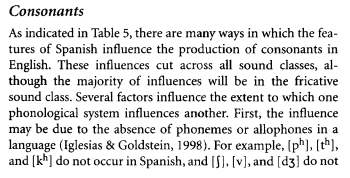
\includegraphics[scale=0.5]{imagenes_investigacion/consonantes1.png}
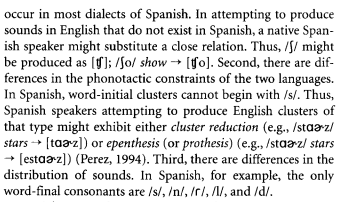
\includegraphics[scale=0.5]{imagenes_investigacion/consonantes2.png}
\end{center}

Visto desde nuestra perspectiva, una persona que aprende una nueva lengua, realiza una aproximación entre los fonos conocidos y los fonos `objetivo' de la nueva lengua.

De manera similar el ingles carece del fono vibrante múltiple alveolar sordo /\textipa{r}/ y dado que el fono /\textipa{R}/ ya estaba siendo utilizado, no podíamos realizar un mapeo tan directo. Como sulución tomamos la mitad de los fonos /\textipa{R}/ y los remplazamos con /\textipa{r}/. Un problema similar surge del fono /g/, que si bien este existe en ingles, al utilizarlo para sintetizar oraciones sonaba muy alienigena. Con el objetivo de suavizar el sonido tomamos el fono de la /g/ y lo mapeamos a un fono que no fuera utilizado y tomamos los fonos etiquetados con /hh/ del ingles y los remplazamos con el /g/ del castellano.

Aquellos fonos que consideramos suficientemente disimiles del castellano, como es el caso de la /sh/, /z/, etc los mapeamos a caracteres que no interfirieran para el entrenamiento ya que no los utilizaremos para la sintesis.

Utilizando estos fonos a la hora de entrenar nos permite sintetizar oraciones en castellano, aunque como es de esperar, dado que el corpus de entrenamiento es tan disimilar de las oraciones que queremos sintetizar, donde tanto las combinaciones de fonemas, las reglas prosodicas y las acentuaciónes vocalicas son distintas, los audios sitetizados resultan incomprensibles y de muy baja calidad

% mapeo utilizado mostrar.
% el etiquetado de cmu\_arctic es en ingles y mapeando al castellano.

\section{Interpolación Entre Modelos}
Una vez generados ambos modelos con el mismo repertorio fonético procedemos a experimentar y evaluar de manera informal la efectividad del método.

Para ello tomamos el modelo generado por \textit{loc1\_pal} y lo interpolamos con \textit{CMU-ARCTIC-SLT} con diferentes pesos entre ellos.

Para grados cercanos al $90\%$ de castellano - $10$ de ingles obtenemos los resultados esperables: las oraciones sintetizadas tienen un marcado acento castellano. Así mismo, en el otro extremo, $10\%$ de castellano - $90\%$ de ingles, la vos sintetizada, al igual que lo que se describió en el apartado anterior, la voz presenta problemas fonéticos graves, haciendo que las oraciones resultaran poco naturales y difíciles o imposibles de comprender. En el medio de la interpolación, $70\%$ de castellano - $30\%$ de ingles y $40\%$ de castellano - $60\%$ de ingles, podemos apreciar resultados mas cercanos a los esperados, pudiendo apreciar en las oraciones sintetizadas detalles distintivos como el fono /\textipa{R}/ mas suavizada, o pronunciación de vocales mas abiertas, pero aun conservando cierto grado de inteligibilidad.

Dado que HTS modela de manera conjunta la acústica y la prosodia, también pudimos apreciar en las oraciones sintetizadas cierta prosodia no familiar que también podría ser adjudicada a un hablante extranjero.  

Como un efecto colateral de la interpolación que pudimos apreciar es que cuanto mas cercano esta el grado de interpolación al modelo en castellano, las características fonéticas se asemejan mas a la de las oraciones del corpus \textit{loc1\_pal}, mientras que de manera análoga, cuanto mas grado de ingles tiene, la voz se asemeja a \textit{CMU-ARCTIC-SLT}. Si bien esto no es un defecto importante, con el motivo de cambiar el menor numero de variables en la experimentación sería deseable que la voz no presentara distintas características para distintos grados de interpolación.

Como una posible solución surge la posibilidad de utilizar Speaker-Adaptative Training sobre uno de los modelos.

\section{Speaker-Adaptative Training}
El Speaker-Adaptative Training técnica permite tomar un modelo ya entrenado y adaptarlo para asimilar características de un nuevo hablante. Esta técnica nace de la idea que construir un corpus de datos es costoso tanto en espacio de almacenamiento, tiempo de grabación y etiquetado, por lo que resulta mas económico generar una nueva voz sintética a partir de un modelo bien generado y adaptándolo luego con características del nuevo corpus.

Nuestro objetivo para este trabajo es utilizar esta herramienta para aproximar las características de uno de los hablantes al otro para que sus identidades fueran indistinguibles.

Como prueba de concepto se tomó el corpus \textit{CMU-ARCTIC-SLT} y se le realizó Speaker Adaptation junto con \textit{loc1\_pal} utilizando la demo presente en la sección de descargas de HTS para el entrenamiento. Las pruebas no son concluyentes ya que las oraciones sintetizadas no solamente pierden la identidad del hablante original sino también sus características fonéticas. Si bien existen indicios que indican que es posible generar un modelo con las características deseadas, dada la complejidad del método y los largos periodos que son necesarios para entrenar un modelo ($36$ horas aproximadamente) decidimos abandonar este camino y continuar con la fase de experimentación.

\section{Herramientas}
En esta sección presentamos las herramientas y los comandos con los que se realizó el preentrenamiento, el entrenamiento y la generación de oraciones para la tesis.

\subsection{Festival y Festvox: Generación de transcripciones fonéticas}

Festival \cite{festivalDownload} es un framework que permite sintetizar habla. Además posee una gran variedad de APIs para el procesamiento de audios y generación de nuevos sistemas TTS. Festvox \cite{festvoxDownload} a su vez expande sobre Festival, agregando todavía más herramientas relacionadas a la síntesis y generación de modelos, que van desde la generación de modelos prosódicos, hasta etiquetado automático de corpus.

Para este trabajo utilizamos Festival y Festvox para generar las oraciones requeridas tanto para el entrenamiento como para la síntesis de audios. Estas transcripciones consisten en una lista de fonos dividida en segmentos temporales y datos contextuales tales como la cantidad de sílabas en la palabra siendo transcrita, fonos que preceden y proceden al actual, etc. A modo de guía, a continuación mostraremos cómo utilizamos estas herramientas para generar las transcripciones fonéticas deseadas usando EHMM alignment.

Primero tenemos que generar un archivo \textit{txt.done.data} donde estén los nombres de cada archivo de audio y su transcripción grafémica. Por ejemplo, en el siguiente recuadro podemos ver un extracto del archivo generado para SECYT\_mm utilizado para este proceso:

\begin{tcolorbox}
( SECYT\_mm\_1\_335 ``Algunos dicen gamba en vez de pierna'' )

( SECYT\_mm\_1\_29 ``El conjunto de las escenas se reitera en el galpón'' )

( SECYT\_mm\_1\_361 ``Lluvia con truenos en Medellín'' )

( SECYT\_mm\_1\_619 ``Rendían pleistecía vikingo conquistador'' )

( SECYT\_mm\_1\_110 ``Llueve sobre las piedras de la pared'' )

( SECYT\_mm\_1\_102 ``Las etapas del desarrollo infantil difieren según el niño'' )

\end{tcolorbox}

En este trabajo utilizamos Festival 2.4 \cite{festivalDownload}, Festvox 2.7 \cite{festvoxDownload} y speech\_tools 2.4 \cite{speechToolDownload} para la generación de transcripciones fonéticas. Para poder utilizarlos agregamos las siguientes variables de entorno en nuestro PATH:

\begin{tcolorbox}
export PATH=/project/festival/bin:\$PATH

export PATH=/project/speech\_tools/bin:\$PATH

export FESTVOXDIR=/project/festvox

export ESTDIR=/project/speech\_tools
\end{tcolorbox}

Luego generamos los directorios, scripts y archivos necesarios para generar una nueva voz:
%referencia
%https://github.com/zeehio/festvox/blob/master/src/clustergen/setup_cg
\begin{tcolorbox}
\$FESTVOXDIR/src/clustergen/setup\_cg uba es SECYT\_mm
\end{tcolorbox}

En la nueva estructura de archivos generada, copiamos los audios en la carpeta wav/ y el archivo \textit{txt.done.data} previamente generado en la carpeta etc/.

Además en los archivos 

\begin{tcolorbox}
festvox/uba\_es\_\_cg.scm 

festvox/uba\_es\_\_clunits.scm
\end{tcolorbox}

\noindent es necesario cambiar las dependencias 

\begin{tcolorbox}
(require 'uba\_es\_\_phoneset)

(require 'uba\_es\_\_lexicon)
\end{tcolorbox}

\noindent que contienen los símbolos fonéticos del español de España, por estas otras:

\begin{tcolorbox}
(require 'uba\_es\_\_phoneset\_mex)

(require 'uba\_es\_\_lexicon\_mex)
\end{tcolorbox}

\noindent que contienen el conjunto de símbolos fonéticos del español mexicano, que se aproximan mucho a los del castellano rioplatense (no contiene [th], por ejemplo).

Finalmente, corriendo los siguientes comandos:

\begin{tcolorbox}
./bin/do\_build build\_prompts

./bin/do\_build label

./bin/do\_build build\_utts
\end{tcolorbox}

\noindent se realizará el proceso de alineamiento y transcripción automática. Una vez finalizado se habrán generado las transcripciones fonéticas con formato .utt en el directorio festival/utts, que entre otra metadata tiene codificados los fonos de la oración, sus principios y sus finales.

De manera análoga, esta herramienta permite crear partituras utilizadas para la síntesis. Simplemente generando un archivo \textit{txt.done.data} con oraciones que se quieran sintetizar, y corriendo el script

\begin{tcolorbox}
./bin/do\_build build\_prompts ./synth/txt.done.data
\end{tcolorbox}

En la carpeta utt gen/prompt-utt se habrán generado los .utt necesarios para la síntesis.


\subsection{HTS}


HTS \cite{hts} es un framework de entrenamiento y síntesis de sistemas TTS basado en HMMs que modela simultáneamente la duración, el espectro (mel-cepstrum) y la frecuencia principal ($f0$) utilizando una combinación de HMMs.

\begin{figure}
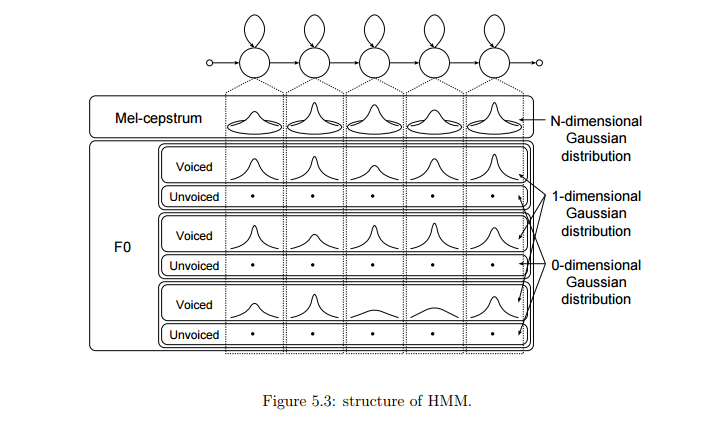
\includegraphics[scale=0.5]{imagenes/hmm.png}
\caption{Estructura de un HMM (tomado de \cite{phoneticAndProsodic}, página 41)}
\label{hmmStructure}
\centering
\end{figure}

La Figura \ref{hmmStructure} resume la estructura de un HMM usado para síntesis del habla. El espectro y la frecuencia fundamental son modelados en paralelo usando vectores separados. En particular el espectro es modelado como un vector de Gaussianas $n$ dimensional, mientras que la frecuencia principal es modelada como un conjunto de vectores de Gaussianas de dimensión uno y cero.

Al mismo tiempo HTS toma la decisión de modelar la información prosódica dentro de este mismo framework. Para esto, las distribuciones para el espectro, la frecuencia principal y las duraciones son clusterizadas independientemente utilizando la información contextual extraída de los audios de entrenamiento. A modo ilustrativo en la Figura \ref{hmmTree} se muestra una esquematización de un HMM resultante, utilizando árboles de decisión para clusterizar los datos. Notar que cada hoja del árbol resultante coincide con un vector $n$ dimensional de Gaussianas o un conjunto de vector de Gaussianas de dimensión cero y uno, según corresponda al espectro o a la frecuencia principal.

\begin{figure}
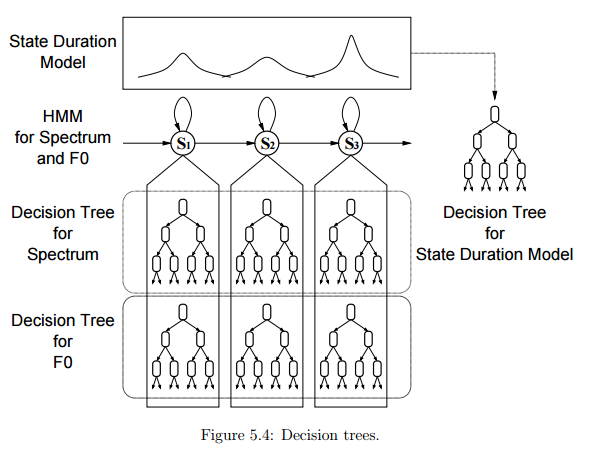
\includegraphics[scale=0.5]{imagenes/hmmContext.png}
\caption{Esquema HMM generado utilizando árboles de decisión (tomado de \cite{phoneticAndProsodic}, página 45)}
\label{hmmTree}
\centering
\end{figure}
%hablar de los distintos tipos de clusters?

Si bien existen muchas maneras de clusterizar el conjunto de fonos, que pueden variar desde algoritmos simples hasta técnicas que utilicen redes neuronales, para este trabajo todos los entrenamientos y clusterizaciones de datos se realizaron con árboles de decisión. 

Por otro lado, como información contextual para el entrenamiento se tomaron los dos fonos por anteriores y posteriores a cada fono y la siguiente información fonética.

\begin{itemize}
\item Modo de articulación del fono:
\begin{itemize}
	\item \TODO
\end{itemize}
\item Punto de articulación del fono:
\begin{itemize}
	\item \TODO
\end{itemize}
\item La perspectiva articulatoria (anterior, central o posterior).
\item Si el fono es una vocal o una consonante.
\item En caso de ser una vocal, a que categoría pertenece: por ejemplo para el fono $[i]:${$i$ (no acentuada), $i0$ (diptongo), $i1$ (acentuada)}.
\item En caso de ser una vocal, su redondeamiento vocálico.
\item En caso de ser una consonante, si es débil o fuerte.
\end{itemize}

De esta manera HTS espera tener una voz más dinámica, que para diferentes valores contextuales darán diferentes modelos acústicos para cada fono.

En la Figura \ref{genTree} se muestra el resultado de un fragmento de uno de los árboles de decisión generado para modelar la duración de un fono. En base a este modelo, el sistema podrá inferir, por ejemplo, que si el fono actual no es nasal (C-Nasal) seguido de un stop (R-Stop), que no es el fono $l$ estará modelado por función de probabilidad Gaussiana definida en $dur\_s2\_7$.

\begin{figure}
\begin{center}
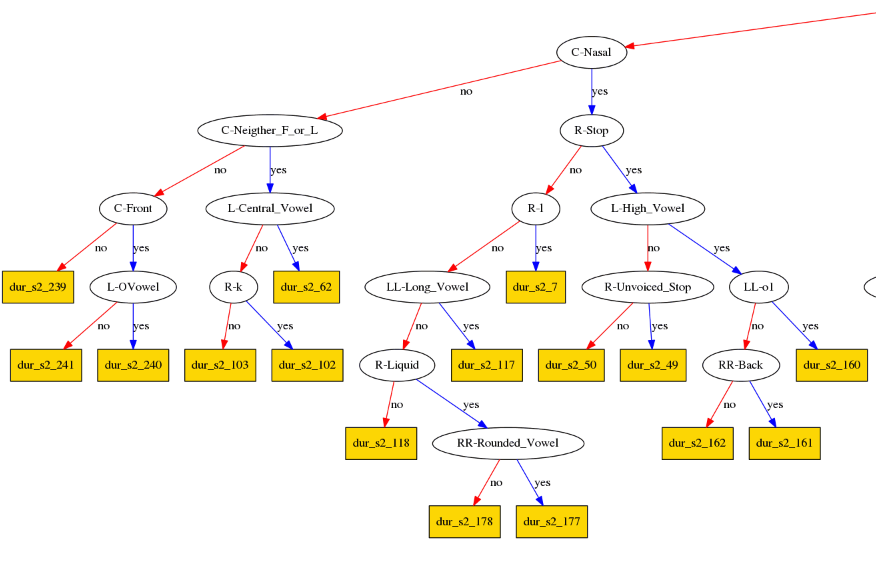
\includegraphics[scale=0.4]{imagenes/arbolDeDesicionTesis.png}
\caption{Árbol de decisión generado a partir de los datos para la duración de un HMM}
\label{genTree}
\end{center}
\end{figure}

En las primeras iteraciones del desarrollo no contábamos con la información acústica, por lo que se generaron modelos carentes de información contextual. En estos primeros modelos se pudo apreciar una calidad muy inferior en los audios generados, sonando estos sumamente metálicos y carentes de prosodia. Esto se debía, posiblemente, a que los árboles de decisión no tenían información contextual suficiente para ser construidos de manera efectiva, resultando en una mala generalización y malos audios sintetizados. Tras agregar los factores contextuales y realizar algunas pruebas de concepto, pudimos comprobar que las voces sonaban con mucha mejor calidad.


\subsection{Entrenamiento} \label{entrenamientoHTS}

Desde un punto de vista puramente técnico, utilizar HTS para entrenar un modelo es bastante sencillo. Asumiendo que todos los paquetes necesarios fueron instalados, es posible entrenar una nueva voz adaptando los scripts disponibles en la página de descargas de HTS.

Para ello, reemplazamos los audios en la carpeta data/raw con aquellos que se quieran utilizar y los utts correspondientes previamente generados. Además, como adelantamos en la sección anterior, le indicamos a HTS qué información contextual se utilizará para la clusterización, por lo que es necesario modificar el archivo data/questions/questions\_qst001.hed con la información contextual apropiada para una voz en castellano. En el apéndice \ref{apendiceQuestions} \completar se presenta el archivo utilizado para Loc1\_pal.

Una vez finalizadas estas modificaciones, en la carpeta data/ de la demo puede iniciarse el pre-entrenamiento de la siguiente manera:

\begin{tcolorbox}
make
\end{tcolorbox}

\noindent Esto extraerá features acústicos del audio y construirá los archivos de entrenamiento, entre otras cosas. Finalmente para dar comienzo al entrenamiento, ejecutamos en la carpeta raíz:

\begin{tcolorbox}
perl scripts/Training.pl scripts/Config.pm $>$ train.log 2$>$ err.log
\end{tcolorbox}

Una vez que se completa el entrenamiento, podemos encontrar en la carpeta voices/qst001/ver1 el modelo generado (.htsvoice).

Para este trabajo todos los audios usaron sampling rate de $48$kHz, precisión de $16$bits, mono. Además HTS requiere que explicitemos un rango de extracción para la frecuencia fundamental de la voz. Tanto para \textit{SECYT-mujer} como para \textit{Loc1-Pal} el rango utilizado utilizado fue desde $100$hz hasta $350$hz, mientras que para \textit{CMU-ARCTIC} el rango de extracción fue desde $110$kHz hasta $280$kHz.

Estos parámetros y muchos otros pueden ser configurados fácilmente corriendo

\begin{tcolorbox}
./configure
\end{tcolorbox}

\noindent en la carpeta raíz del proyecto. En la próxima sección detallaremos como utilizar varios .htsvoice generados para mezclar y sintetizar una nueva voz.

\subsection{HTS\_engine} \label{interpolationTeory}

Finalmente, para generar voces con acento extranjero se utilizó hts\_engine. Esta herramienta, entre otras cosas, permite interpolar entre varios modelos, para producir un nuevo modelo con una mezcla de la carga fonética y prosódica. Esto nos brinda un gran rango exploratorio y nos permite ajustar la carga fonética de los modelos entrenados previamente para cumplir con nuestro objetivo de sintetizar habla en castellano con acento inglés.

A grandes rasgos, la interpolación consiste en tomar los vectores generados anteriormente durante el entrenamiento e interpolar sus funciones de densidad Gaussianas para obtener una nueva. En la Figura \ref{spekerInterpolationImagen} (extraída del trabajo \cite{SpekerInterpolationRef}) puede verse la interpolación de $N$ HMMs, cada uno con peso arbitrario $a_1$, $a_2$, ..., $a_N$, que generan un nuevo modelo $\Lambda$.

\begin{figure}
\begin{center}
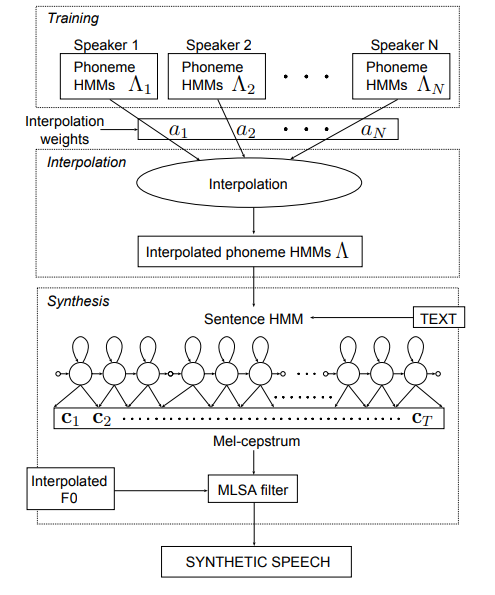
\includegraphics[scale=0.4]{imagenes/speakerInterpolation.png}
\caption{Block diagram of speech synthesis system with speaker interpolation. (tomado de \cite{phoneticAndProsodic}, página $70$) }
\label{spekerInterpolationImagen}
\end{center}
\end{figure}

Una vez obtenido el nuevo HMM, el proceso de síntesis puede ocurrir como para cualquier otro modelo, ilustrado en la etapa de síntesis de la figura. El procedimiento para sintetizar una nueva oración es bastante simple. Asumiendo que todas las dependencias fueron instaladas de manera correcta, con el siguiente comando es posible utilizar los modelos generados en \textit{cmu\_us\_arctic\_slt.htsvoice} y \textit{models/loc1\_pal.htsvoice} para interpolar con peso $0.7$ y $0.3$ respectivamente, generar un nuevo modelo y sintetizar la oración presente en el archivo in.lab.

\begin{tcolorbox}
hts\_engine -m models/cmu\_us\_arctic\_slt.htsvoice -m models/loc1\_pal.htsvoice -i 2 0.7 0.3 -ow out.wav in.lab
\end{tcolorbox}

Esta herramienta permite además modificar el pitch, la duración del audio y otros aspectos de la síntesis. La documentación completa puede encontrarse en la pagina web: http://hts-engine.sourceforge.net/.
\pagebreak
%Experimentación
\section{Experimentación}

En esta sección intentamos validar que el habla sintetizada por los modelos generados realmente puede ser identificada como perteneciente a personas de habla inglesa, y al mismo tiempo evaluar sus grados de inteligibilidad. Para eso se condujo una encuesta perceptual donde a cada participante se le presentó una oración sintetizada con distintos grados de mezcla de español e inglés y se le pidió que la transcribiera y que intentara identificar la nacionalidad del hablante. 

La encuesta se realizó a través de Internet, con el mismo set de instrucciones para todos los participantes y pidiendo como requisito la utilización de auriculares. Cada participante podía contestar un máximo de $5$ veces, presentándoles siempre oraciones distintas.

Nos propusimos como objetivo conseguir $5$ respuestas para cada uno de los $50$ audios sintetizados, momento en el cual se cerró la posibilidad de contestar. Se llevó a cabo desde el $18$ de octubre de $2017$ hasta el primero de diciembre del mismo año, tiempo durante el cual fue publicitada en distintas redes sociales y listas de emails de distintas facultades.

Con el objetivo de no influir en las respuestas de los participantes, se procuró darles la información mínima indispensable para completar la encuesta. Por este motivo, en ningún momento de la encuesta se especifica el objetivo real de la misma. Con la intención de homogeneizar la muestra, fue requisito obligatorio utilizar auriculares para la encuesta. También se le pidió a cada participante que la realizara en un lugar silencioso y tranquilo.

A continuación, describimos la forma en que se construyeron los audios usados en esta evaluación y la interfaz de la encuesta. Luego mostramos los datos demográficos  obtenidos. Más adelante, continuamos con un análisis exhaustivo de inteligibilidad y origen atribuido a las oraciones.
Por último, para evaluar la hipótesis original, compondremos estos dos ejes para dilucidar el grado de validez de los resultados.

\section{Audios sintetizados}

Para evitar que el participante pudiera deducir las palabras de los audios a partir de las palabras vecinas, las mismas fueron generadas de manera \textit{semánticamente impredecible}. Esto significa que a partir de una lista de sustantivos, adjetivos, determinantes y verbos se generaron oraciones de manera aleatoria con la siguiente estructura:

$$\textnormal{\textit{Determinante Adjetivo Sustantivo Verbo Determinante Sustantivo}}$$

Luego, para asegurarnos de estar cubriendo todos los posibles fonos del castellano, las oraciones fueron modificadas para ser fonéticamente balanceadas. Esto significa que incluimos entre cinco y diez veces cada fono perteneciente a una consonante (del castellano) y al menos veinte veces cada fono perteneciente a una vocal.

Los oraciones generadas fueron:

\begin{itemize}
\item Oración 1: Mi montaña aguileña recorrió la esquina.
\item Oración 2: Aquel fuerte vidrio prefirió aquel botón.
\item Oración 3: Este enjoyado juez comprará nuestro corchete.
\item Oración 4: Tu estrecho posavasos gritó la fechoría.
\item Oración 5: Nuestro nublado tigre concluyó a este chupetín.
\item Oración 6: Su profundo riñón apoyó a Julio.
\item Oración 7: El frío churrasco oyó lo de Polonia.
\item Oración 8: Las acongojadas cotorras sonrieron a mi círculo.
\item Oración 9: Ese gruñón perro prometió a esos cuñados.
\item Oración 10: El nudillo argentino perdió su vaso.
\end{itemize}

Para cada una de estas diez oraciones se varió el nivel de mezcla entre $30\%$ de inglés + $70\%$ castellano hasta $70\%$ de inglés + $30\%$ de castellano, con $10\%$ de incremento. De esta manera, para cada oración hay $5$ mezclas diferentes, lo que hace un total de $50$ audios sintetizados diferentes.

\section{Interfaz}\label{interfaz}

En esta sección se presenta la interfaz utilizada para realizar la encuesta junto con las decisiones de diseño más relevantes. En la Figura \ref{personalData} se presenta la página con la que todos los participantes fueron recibidos. A fin de conocer de manera general la demografía encuestada, a cada participante se le pidió que indicara el rango correspondiente a su edad, yendo desde $18$ a $25$, $26$ a $35$, y así de diez en diez.

\begin{figure}[htp]
\begin{center}
\fbox{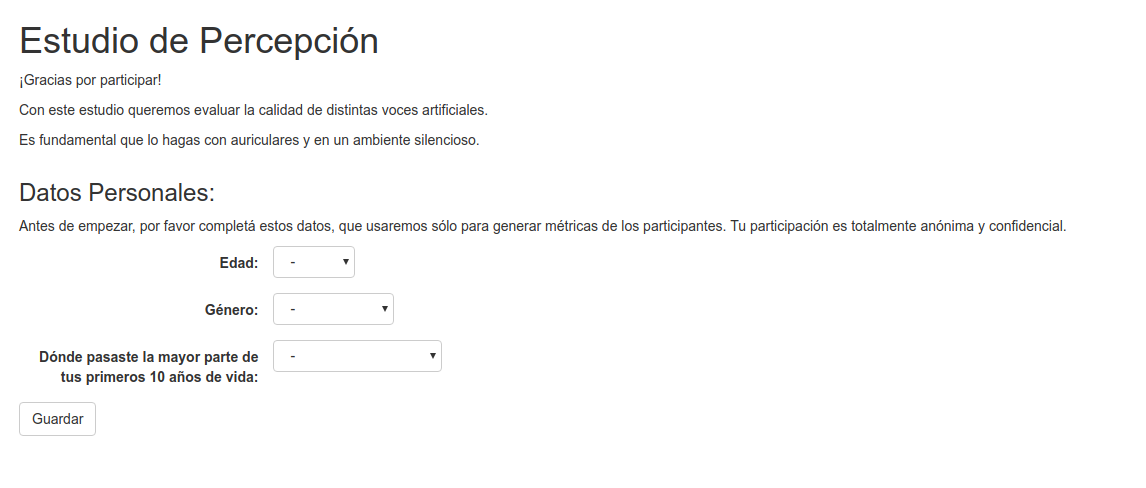
\includegraphics[scale=0.6]{estudio_online/estudio1.png}}
\end{center}
\caption{Primera pantalla de la encuesta, en la cual se recaban datos personales}
\label{personalData}
\end{figure}

Se le pidió, además, que indicara su género: ``masculino'', ``femenino'', ``otro'', ``no contesta'' y la provincia donde pasó la mayor parte de sus primeros diez años de vida. Consideramos que estos datos son importantes para el estudio ya que dependiendo de ellos los resultados variarán indefectiblemente. Por ejemplo la transcripción que obtendremos de un participante de $50$ años de Capital Federal será distinta a la de alguien de $18$ años de Córdoba. El diferente uso de los alofonos, modismos y variantes prosódicas y capacidades auditivas jugarán un papel importante en la interpretación de la oración y la apreciación del origen del hablante.

\begin{figure}
\begin{center}
\fbox{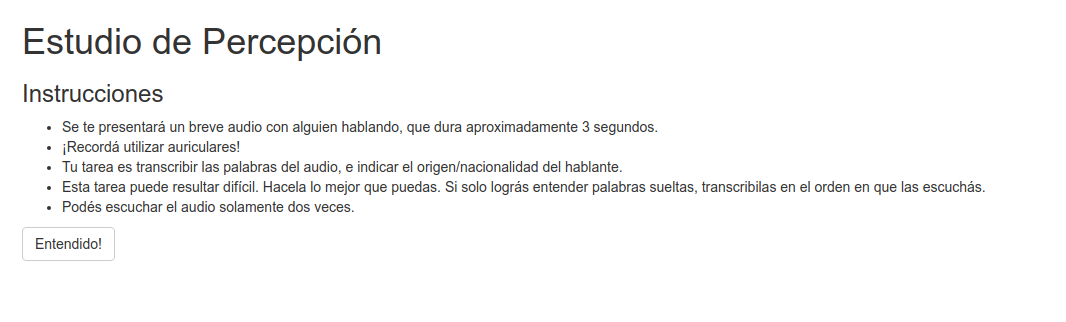
\includegraphics[scale=0.6]{estudio_online/estudio2.png}}
\end{center}
\caption{Pantalla con las instrucciones de la encuesta}
\label{instrucciones}
\end{figure}

Como puede verse en la Figura \ref{instrucciones}, una vez completados estos datos, a cada participante se le presentó otra vista con las instrucciones específicas para completar la encuesta. Una vez presionado el botón de ``Entendido!'' se les presentó el primer audio, que podían escuchar un máximo de $2$ veces, una caja de texto libre donde ingresar la transcripción del mismo y una caja de texto libre donde podían escribir cual consideraban que era el origen de la nacionalidad correspondiente a la voz, como puede apreciarse en la Figura \ref{transcripcion}.

\begin{figure}
\begin{center}
\fbox{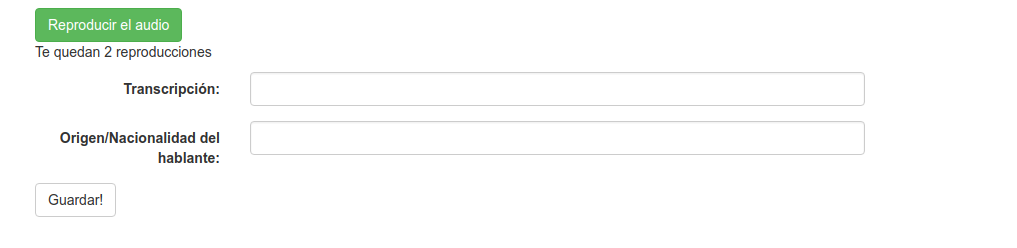
\includegraphics[scale=0.6]{estudio_online/estudio3.png}}
\end{center}
\caption{Pantalla de transcripción}
\label{transcripcion}
\end{figure}

Una vez guardada la respuesta, se le preguntó si quería continuar transcribiendo otro audio. En caso de haber completado cinco audios, se le mostró un mensaje indicando que ya podía cerrar la encuesta:

\begin{center}
\fbox{
¡Muchas gracias por tu participación! Ya podés cerrar la ventana del navegador.}
\end{center}

\pagebreak
\section{Resultados}

A modo de introducción, comenzaremos esta sección mostrando los datos demográficos obtenidos. Mas adelante, continuaremos con un análisis mas exhaustivo de inteligibilidad y por separado se realizará otro análisis respecto a la nacionalidad atribuida a las oraciones. Por último para evaluar la hipótesis original, compondremos estos dos ejes para dilucidar su grado de validez.

\section{Datos demográficos}

Se encuestaron $109$ participantes de los cuales se obtuvieron $352$ resultados.

Del total de participantes, $49$ pertenecían al rango comprendido entre $18$ y $25$ años, $43$ estaban en el rango $26$-$35$. $17$ de los participantes eran mayores a $35$ años (fig. \ref{genero}).

\begin{figure}
\centering
\begin{subfigure}{.5\textwidth}
  \centering
	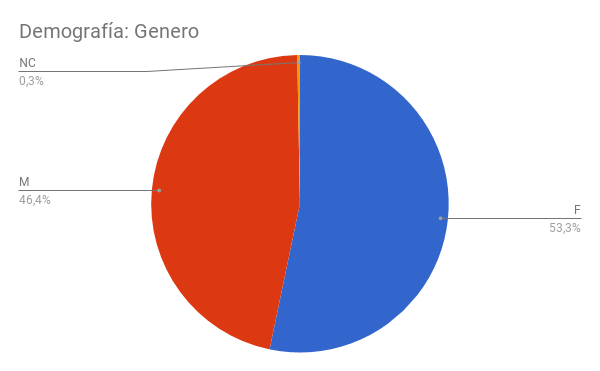
\includegraphics[width=.4\linewidth]{datosDemograficos/genero.png}
  \caption{A subfigure}
  \label{fig:sub1}
\end{subfigure}%
\begin{subfigure}{.5\textwidth}
  \centering
	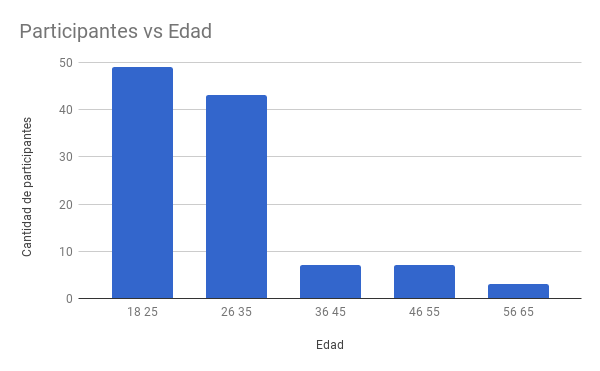
\includegraphics[width=.4\linewidth]{datosDemograficos/edad.png}
  \caption{A subfigure}
  \label{fig:sub2}
\end{subfigure}
\caption{A figure with two subfigures}
\label{fig:test}
\end{figure}

Con respecto al genero de los participantes, $187$ respuestas fueron brindadas por participantes del genero femenino mientras que $163$respuestas fueron brindadas por participante del genero masculino (fig. \ref{edad}).

En los datos referentes a la región en que cada participante pasó su infancia puede verse una predominancia de personas del Gran Buenos Aires con $45\%$, seguido por un $30\%$ que pasaron su infancia en la Capital Federal. Menos del $25\%$ pertenece al resto de las provincias Argentinas. Además, $10$ personas contestaron que se criaron fuera del país (fig. \ref{distTerritorial}).

\begin{figure}
\begin{center}
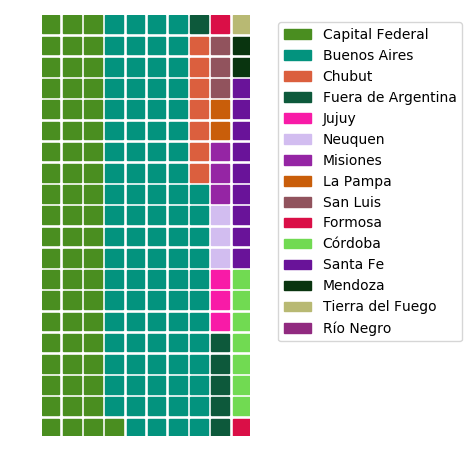
\includegraphics[scale=0.8]{datosDemograficos/infancia.png}
\end{center}
\caption{Distribución Territorial}
\label{distTerritorial}
\end{figure}

\section{Inteligibilidad}

A continuación intentaremos medir la inteligibilidad de cada una de las oraciones en base a las respuestas obtenidas por los participantes. Para ello tomaremos la oración transcripta por los participantes y mediremos cuán lejos o cerca está de la oración original. 

Para esto utilizaremos la distancia de Levenshtein, que consiste en calcular la menor cantidad posible de inserciones, remociones o reemplazos de caracteres posibles que son requeridos para transformar la oración transcripta por un participante en la oración objetivo. Así por ejemplo, para transformar \textit{cosa} en \textit{cal} se requieren $3$ transformaciones: reemplazar \textit{o} por \textit{a} final, reemplazar \textit{s} por \textit{l} y remover la \textit{a} por lo que la distancia de Levinshtein entre estas dos palabras es de $3$. Además, se considerará un remplazo cualquier acento, por lo que \textit{á} y \textit{a} tendrán distancia $1$ pero no así el reemplazo de mayúsculas y minúsculas, por lo que \textit{a} y \textit{A} tendrán distancia $0$.

En la figura \ref{resultadosGenerales} presentamos los resultados generales obtenidos sin ningún tipo de modificación a las transcripciones ingresadas por los sujetos.

\begin{figure}
\begin{center}$
\begin{array}{lll}
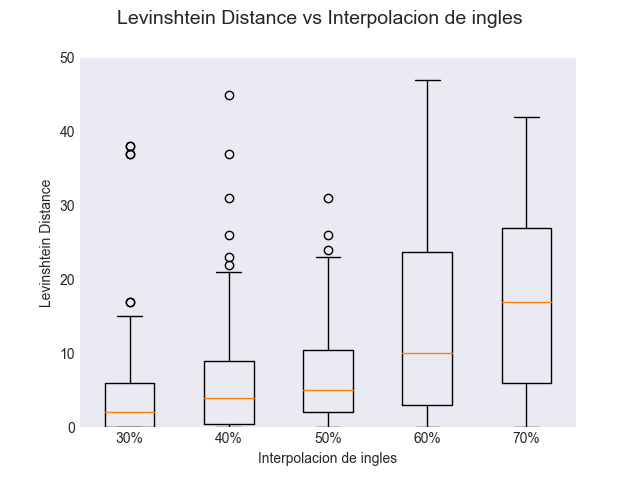
\includegraphics[width=.7\textwidth]{imagenes/plots_raw/general.png}
\end{array}$
\end{center}
\caption{Distancia de Levinshtein para distintos grados de interpolación}
\label{resultadosGenerales}
\end{figure}

Como puede observarse hasta el $50\%$ de mezcla castellano-ingles, la distancia entre el primer y tercer cuartil menor a $10$ caracteres, siendo la media de $5$ caracteres. Pasados el $60\%$ de ingles, se observa un aumento brusco el la distancia intercuartiles, la distancia entre el primer y tercer cuartil pasa a ser cercana a $20$ caracteres, y la media $10$ caracteres en el caso de $60\%$ ingles y $15$ en el caso del $70\%$. En las proximas secciones intentaremos encontrar una explicación intuitiva a estos números.

\section{Problemas en las transcripciones y normalización}

Analizando detenidamente las transcripciones obtenidas pudimos observar algunas fallas sistemáticas que podrían generar ruido en el análisis, por ejemplo algunos de los participantes escribieron de manera diferente las secciones de la oración que no comprendieron. Por citar algunos ejemplos, muchos de ellos escribieron: ``...'', ``....'' o simplemente omitieron la palabra, mientras que una minoría escribió cosas como ``***'', ``???'', ``\textit{blablabla}''. En los casos donde el participante no comprendió ningún segmento de la oración, es común observar expresiones como ``\textit{no entendí nada}'', ``\textit{nada}'', etc.

Por otra parte es común la utilización innecesaria de signos de puntuación. Estos varían desde puntos finales para expresar el final de la oración hasta expresiones de confusión tales como ``(?)''. En un caso extremo, un participante el participante transcribió \textit{``tu estrecho posavasos'', grito la fechoría}, cuando la oración original solo decía \textit{tu estrecho portavasos gritó la fechoría}.
También pueden verse omisiones de acentos y faltas ortográficas en palabras que no presentan ambigüedades, como por ejemplo: ``grunion'' en vez de ``gruñón''.

Todas estas expresiones y modimos tienen como consecuencia directa que la distancia de Levinshtein se vea afectada. Por ejemplo un participante que haya escrito ``\textit{no entendí nada}'' como respuesta devolverá una distancia distinta de aquel que simplemente dejó el campo vacío o de aquel que escribió ``\textit{nada}''.

Con el objetivo de reducir esta varibabilidad en la muestra, se decidió realizar una limpieza de los datos. En esta limpieza buscamos uniformizar los datos para un mejor analisis, intentando mantener siempre el espiritu de la respuesta dada por el participante. De esta manera consideramos que si un participante escribió ``...'' en medio de una oración, lo que quiso decir es que no comprendió parte de la misma. Hubiera sido igual que hubiese escrito la cadena vacía ``'', por ejemplo.

De esta manera consideramos que los siguientes cambios no presentan alteraciones grabes en las respuestas de los participantes:

\begin{itemize}
	\item Corregir ``ni'' por ``ñ'' en la palabra \textit{grunion}.
	\item Remoción de todos los signos de puntuación: comas, puntos, ``(?)''
	\item Reemplazo de oraciones como \textit{blabla}, \textit{no entendí} o cualquier otra expresión que indique ininteligibilidad de una palabra u oración por la cadena vacía ``''.
	\item Corrección de acentos en palabras no ambiguas: \textit{botón}, \textit{prefirió}, \textit{recorrió}, \textit{chupetín}, \textit{riñón}, \textit{gruñón}.
\end{itemize}

Aquellas palabras que presentan ambivalencia, como \textit{concluyó}, no fueron modificadas ya que tanto \textit{concluyó/concluyo} son válidas. El participante podría haber interpretado la palabra con cualquiera de las dos connotaciones cambiando el significado de la interpretación y su distancia de Levinshtein.

Esperamos que esta limpieza nos ayude a disminuir la varianza de los resultados, y así tambien, nos permitirá interpretar de manera mas intuitiva el significado la distancia de Levenshtein en cada caso.

\clearpage

\section{Datos normalizados}

Podemos observar en la figura \ref{generalNormalizado} los nuevos resultados con los datos normalizados. Para $40\%$ y $50\%$ ingles . Para $60\%$ . Para $70\%$ .

\begin{figure}
\begin{center}$
\begin{array}{lll}
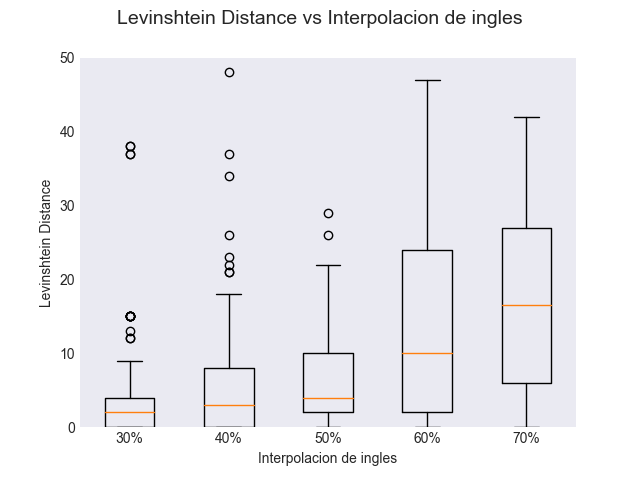
\includegraphics[width=.7\textwidth]{imagenes/plots_normalized/general.png}
\end{array}$
\end{center}
\caption{General Normalizado}
\label{generalNormalizado}
\end{figure}

Con este baseline, podemos ver que para una interpolación de ingles de $30\%$, $96$ de los $106$ participantes obtuvieron una distancia menor a los $10$ caracteres en la transcripción del texto, mientras que los $10$ restantes una distancia mayor a los 10 caracteres. Podemos ver además que la distancia entre el primer y tercer cuartil es menor a $5$ caracteres con una media cercana a $2$ 

Para la mezcla $40\%$ ingles - $60\%$ castellano, de un total de $67$ participantes, $57$ anotaron una distancia de Levinshtein menor a diez caracteres, $7$ una distancia entre $10$ y $30$ caracteres y $3$ una distancia mayor a $30$. La distancia intercuartil es de aproximadamente diez caracteres, con una media muy similar a la mezcla $30\%$ ingles.

Para la interpolación $50\%$ ingles - $50\%$ castellano, de un total de $75$ participantes, $57$ lograron transcribir el audio con una distancia menor a 10 caracteres, mientras que $14$ anotaron una distancia entre $10$ y $20$ caracteres y $4$ una distancia mayor a $20$. De manera similar que para $40\%$ la distancia intercuartil es de aproximadamente diez caracteres y la media es de $3$ caracteres.

Con esta estandarización de los datos, trataremos de darles un peso intuitivo que nos permitan sistematizar el análisis.

Por ejemplo, tomando la oración $8$ de las frases utilizadas en la experimentación: 

\begin{itemize}
	\item ``Las acongojadas cotorras sonrieron a mi círculo''
\end{itemize}

Podemos observar las siguientes transcripciones extraídas de los resultados:

\begin{itemize}
	\item Distancia 0: ``Las acongojadas cotorras sonrieron a mi círculo''
	\item Distancia 10: ``Las acontojadas culturas sonrieron en semicírculo''
	\item Distancia 20: ``Plaza sombreada con sombrero sonrieron en mi círculo''
	\item Distancia 30: ``sonrieron en mi círculo''
	\item Distancia 40: ``círculo''
	\item Distancia 48: ``''
\end{itemize}

Para todas las interpolaciones enunciadas previamente, los errores mas comunes varían desde falta de acentos en palabras como ``concluyó'' hasta faltas de inteligibilidad en palabras con cierta complejidad fonética como ``aguileña'' o ``gruñón''.

Como caso particular la oración $3$: ``este enjoyado juez comprará nuestro corchete'' podemos observar que la mayoría de los participantes cometieron errores al transcribir la palabra ``juez'' que confundieron de manera sistemática con palabras sonoramente similares como ``fue'', y ``enjoyado'' que transcribieron como ``enfollado'', ``enrollado'' y la conjugación exacta del verbo comprar.

Para los grados de interpolación $60\%$ ingles - $40\%$ castellano y $70\%$ ingles - $30\%$ castellano, podemos observar un aumento notable de la variabilidad en las respuestas. Para el primero, de las $70$ respuestas obtenidas, $40$ participantes lograron transcribir el audio con una distancia menor a diez caracteres, $6$ obtuvieron anotaron una distancia entre $10$ y $20$ caracteres, y $24$ transcribieron el audio con distancia mayor a veinte caracteres. La distancia entre el primer y tercer cuartil pasa a ser de $20$ caracteres con una media igual a $10$.

Para $70\%$ ingles - $30\%$ castellano, la diferencia es todavía mas marcada, de los $68$ resultados obtenidos, $28$ lograron transcribir el audio con un buen grado de inteligibilidad, $8$ con un grado medio y $32$ con un grado bajo o nulo de inteligibilidad. La distancia intercuartil se mantiene similar a la de mezcla $60\%$ ingles, aproximadamente $20$ caracteres pero vemos un salto en la media que ahora es de $20$ caracteres.

Consideramos que este salto en la distancia intercuartil puede deberse a dos motivos: El primero es que existen características particulares de los participantes y sus capacidades para discernir palabras, incluso cuando presentan defectos en la pronunciación del hablante. En particular, la oración $4$ (ver figura \ref{oracionCuatro}) muestra cómo para el $70\%$ de ingles - $30\%$ de español en la interpolación, $2$ participantes de los $9$ que realizaron la transcripción, obtuvieron distancias $2$ y $6$ en sus transcripciones.

\begin{figure}
\begin{center}$
\begin{array}{lll}
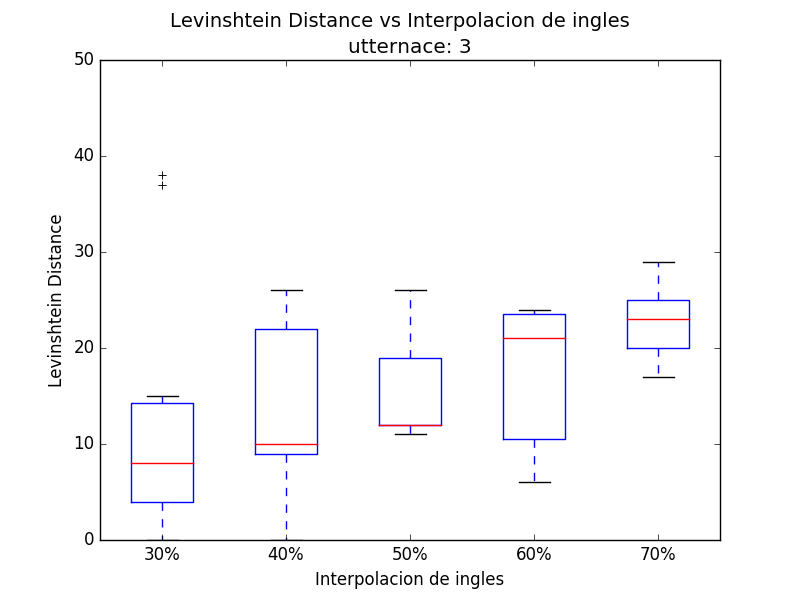
\includegraphics[width=.5\textwidth]{imagenes/plots_normalized/3.png}
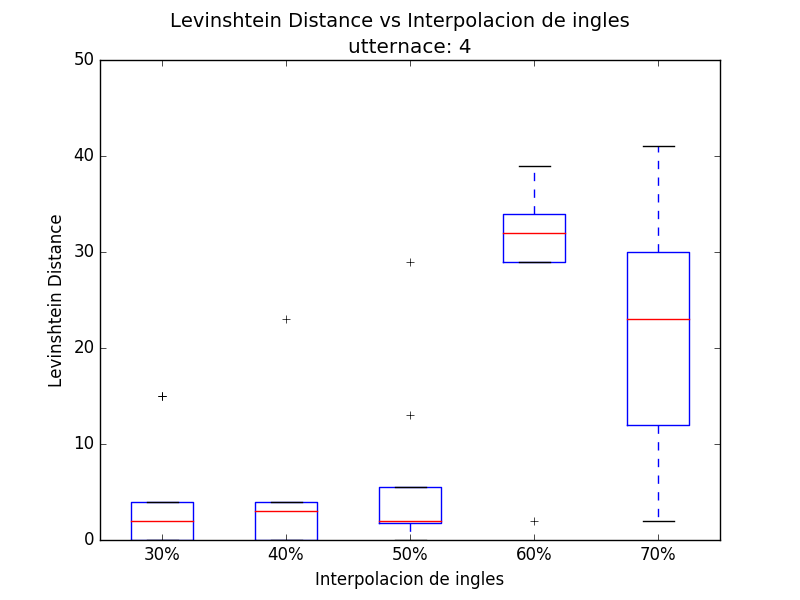
\includegraphics[width=.5\textwidth]{imagenes/plots_normalized/4.png}
\end{array}$
\end{center}
\caption{Oración 4 Normalizada}
\label{oracionCuatro}
\end{figure}

El segundo motivo puede deberse a que existen características particulares de las oraciones o del modelo utilizado para generar la voz que afectan la comprensión del audio: la oración $10$ con $70\%$ de interpolación de ingles - $30\%$ de castellano, en la cual $6$ de los $8$ participantes obtuvieron una buena transcripción del audio con distancia menor a $15$, y la oración $8$, donde, para ese mismo grado de interpolación, todos los participantes transcribieron el audio con distancia de Levinshtein mayor a $20$, parecen demostrar esto. O bien la dificultad de las oraciones es variable o, lo que es todavía mas probable, llegado cierto punto en la interpolación, algunos fonemas empiezan a ``romperse'' o se alejan demasiado del fonema castellano correcto y terminan por disminuir la claridad de la voz.

\begin{figure}
\begin{center}$
\begin{array}{lll}
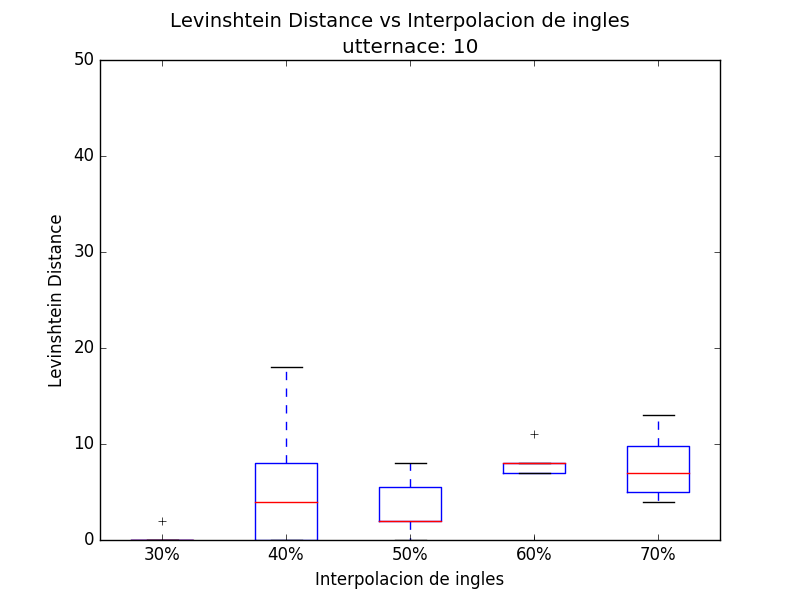
\includegraphics[width=.5\textwidth]{imagenes/plots_normalized/10.png}&
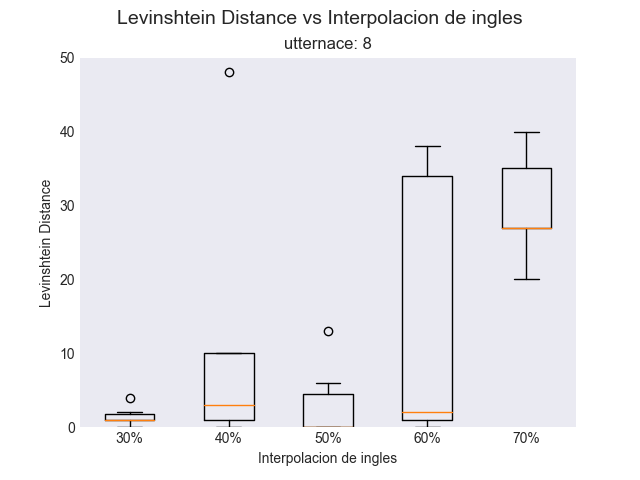
\includegraphics[width=.5\textwidth]{imagenes/plots_normalized/8.png}
\end{array}$
\end{center}
\caption{Oración 10 y 8 Normalizados}
\label{pics:blablabla}
\end{figure}

En conclusión, en esta sección pudimos demostrar que fue posible generar una voz con una distancia menor a $10$ caracteres hasta un $50\%$ de ingles y $50\%$ de castellano. Pasado el $50\%$ de ingles, la variabilidad de las respuestas se vuelve mucho mas grande pudiendo haber participantes que anotan una buena distancia de Levinshtein ($10$ caracteres o menos) hasta algunos que no logran comprender ni siquiera segmentos aislados del mismo (mas de $30$ caracteres).

% \begin{figure}
% \begin{center}$
% \begin{array}{lll}
% 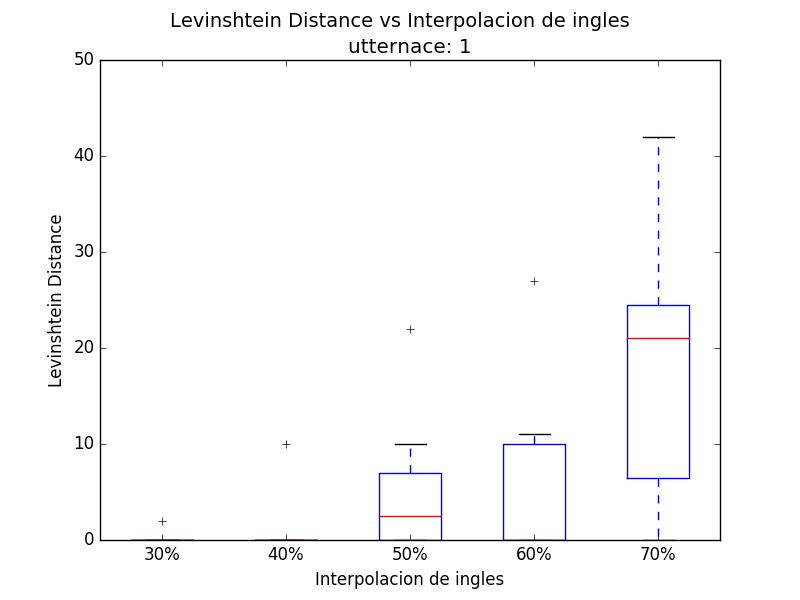
\includegraphics[width=.5\textwidth]{imagenes/plots_normalized/1.png}&
% 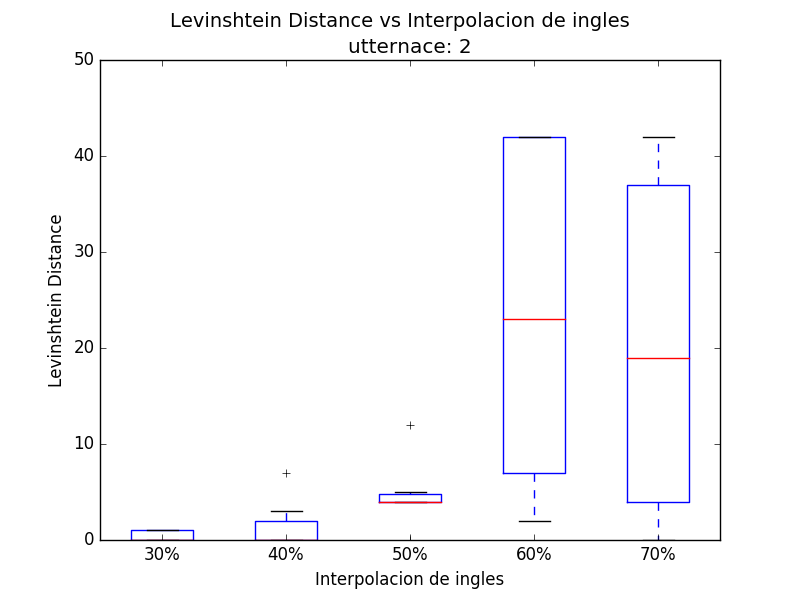
\includegraphics[width=.5\textwidth]{imagenes/plots_normalized/2.png}
% \end{array}$
% \end{center}
% \caption{Utternace 1 y 2 Normalizados}
% \label{pics:blablabla}
% \end{figure}

% \begin{figure}
% \begin{center}$
% \begin{array}{lll}
% 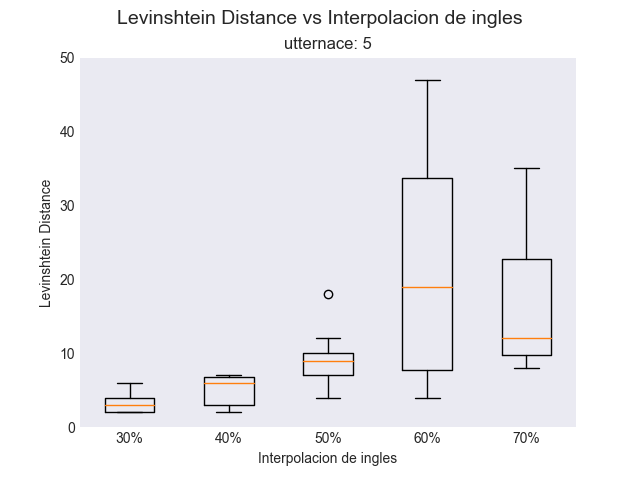
\includegraphics[width=.5\textwidth]{imagenes/plots_normalized/5.png}&
% 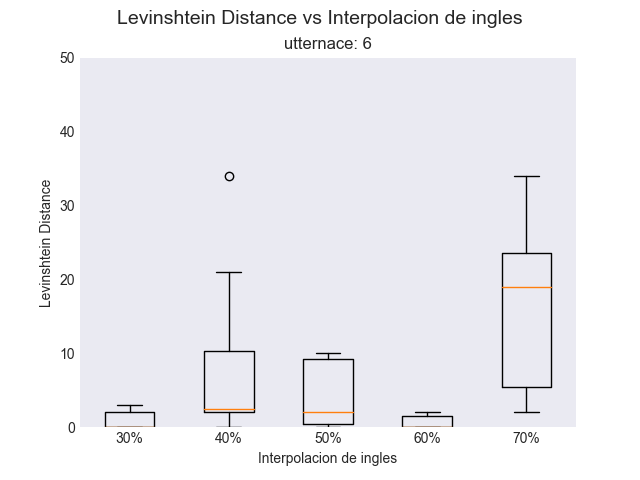
\includegraphics[width=.5\textwidth]{imagenes/plots_normalized/6.png}
% \end{array}$
% \end{center}
% \caption{Utternace 5 y 6 Normalizados}
% \label{pics:blablabla}
% \end{figure}

% \begin{figure}
% \begin{center}$
% \begin{array}{lll}
% 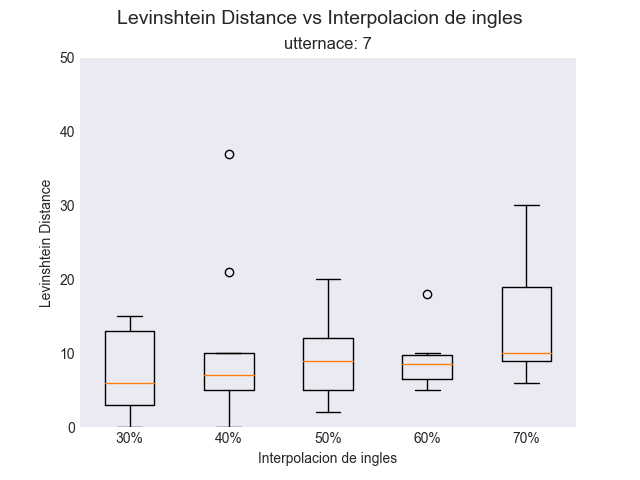
\includegraphics[width=.5\textwidth]{imagenes/plots_normalized/7.png}&
% 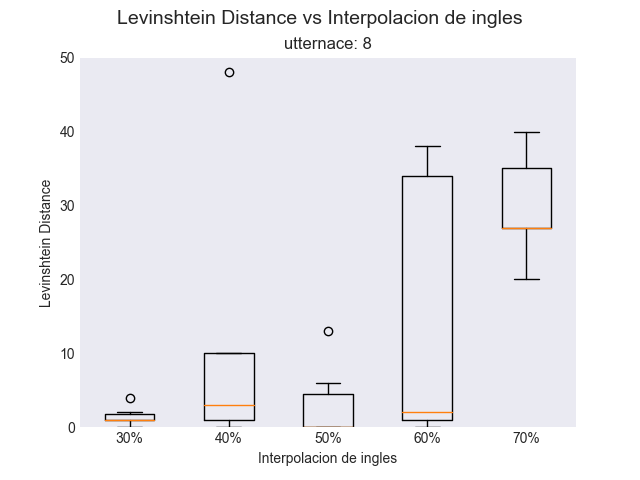
\includegraphics[width=.5\textwidth]{imagenes/plots_normalized/8.png}
% \end{array}$
% \end{center}
% \caption{Utternace 7 y 8 Normalizados}
% \label{pics:blablabla}
% \end{figure}


%Agregar:
% python levinshteinFor.py 0
% Alta int: 96
% Media int: 10
% Baja int: 0
% nula: 4
% python levinshteinFor.py 1
% Alta int: 57
% Media int: 2
% Baja int: 5
% nula: 3
% porque nula? ver esto: parecen ser outliers
% python levinshteinFor.py 2
% Alta int: 57
% Media int: 14
% Baja int: 4
% nula: 0
% python levinshteinFor.py 3
% Alta int: 40
% Media int: 6
% Baja int: 11
% nula: 13
% python levinshteinFor.py 4
% Alta int: 28
% Media int: 8
% Baja int: 20
% nula: 12


\clearpage
\section{Análisis del Órigen Percibido}

En esta sección analizaremos los resultados de los origenes o nacionalidades que los participantes de la encuesta atribuyeron a la voz.

Dado que en esta instancia se le permitió a los participantes ingresar texto libre las respuestas resultaron bastante heterogéneas. Los participantes tomaron la consigna de manera diferente, pudiendo encontrarse respuestas que no pueden ser atribuidas a una nacionalidad. Como ejemplo de algunas respuestas pueden encontrarse cosas como: ``Latino'', ``Anglo'', ``Robot'', ``España (sur)''.

Consideramos que las respuestas de la índole ``robot'', ``es una voz artificial'', no son validas ya que no aportan información para esta investigación.

Por esta razón, en esta instancia decidimos agrupar las respuestas en cuatro grupos:

\begin{itemize}
	\item Hispanoparlate: ``Latino'', ``Argentino'', ``Español'', ``Uruguayo'', ``Centroamericano'', ``Boliviano'', `` Mexicano'',``Colombiano''.
	\item Angloparlante: ``Estadounidense'', ``Ingles'', ``Irlandés'', ``Canadiense'', ``Anglo''.
	\item No sabe/No contesta: ``Robot'', ``no se''.
	\item Otro: ``Ruso'', ``Brasiltiño'' (sic).
\end{itemize}

Con estas agrupaciones, en la figura \ref{analGeneral} presentamos las nacionalidades atribuidas a la voz generada para cada punto de la interpolación.

\begin{figure}
\begin{center}$
\begin{array}{lll}
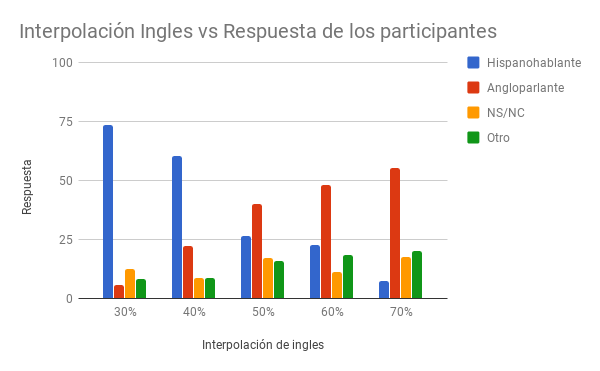
\includegraphics[width=.7\textwidth]{imagenes/nacionalidades/general.png}
\end{array}$
\end{center}
\caption{Análisis General}
\label{analGeneral}
\end{figure}

De estos resultados podemos observar que con $30\%$ de interpolación de ingles, los participantes coinciden en que la voz puede atribuirse a una persona de habla nativa española.

Con interpolación $50\%$ de ingles - $50\%$ de castellano y $60\%$ ingles - $40\%$ castellano, los resultados son similares: aproximadamente en la mitad de las oraciones, mas de la mitad de los participantes consideraron que la voz pertenecía a un anglosajón hablando castellano. Para estos grados de interpolación también podemos observar que en un $80\%$ de las oraciones al menos un $20\%$ de los participantes atribuyen la nacionalidad del hablante a extranjero de origen no anglosajón hablando castellano.

Con $70\%$ de interpolación, en el $80\%$ de las oraciones se puede apreciar que al menos $50\%$ de los participantes dijo que el hablante era de origen anglosajón. Mas aún, en el $40\%$ de las oraciones el $75\%$ de los participantes coincidió que la voz era de angloparlante. También podemos ver que para este grado de interpolación en el $70\%$ de las oraciones ningún participante considera que la voz sea de habla hispana. En el $30\%$ restante, $25\%$ de los participantes o menos consideran que la voz pertenezca a un hispanohablante.

%grafico general mostrando como crece el grado de ingles?

%conclucion mas general: aunque en muchos casos los participantes atribuyeron a la voz como un extrangero no anglosajon, tambien tener en cuenta que se esta intentando identificar la nacionalidad de un hablante con tan solo con una oración como referencia.

Observando las oraciones una por una, podemos observar algunas particularidades. para $40\%$ ingles, puede verse que no hay una votación homogénea. Por ejemplo en la figura \ref{tresNueve} en la oración $3$ el $80\%$ de los participantes coincide que la voz pertenece a un hablante de habla hispana, mientras que en la oración $9$ el $60.00\%$ de los participantes considera que la voz pertenece a un hablante de habla anglosajona.

\begin{figure}
\begin{center}$
\begin{array}{lll}
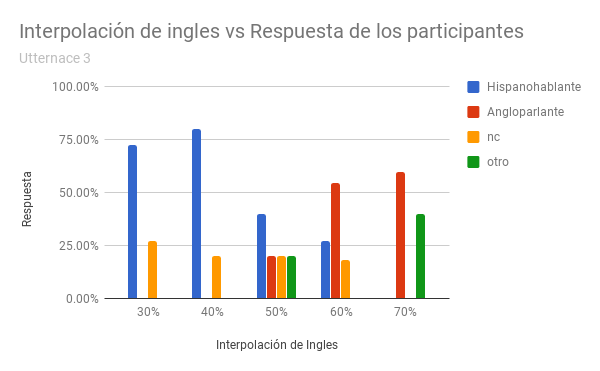
\includegraphics[width=.5\textwidth]{imagenes/nacionalidades/3.png}&
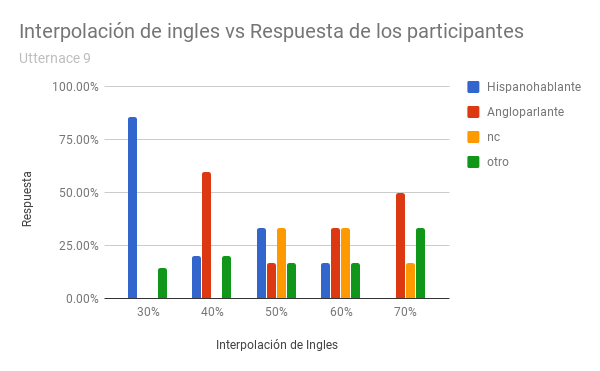
\includegraphics[width=.5\textwidth]{imagenes/nacionalidades/9.png}
\end{array}$
\end{center}
\caption{Oración 3 y 9}
\label{tresNueve}
\end{figure}

Esta gran disparidad de resultados entre distintas oraciones se puede atribuir a las características particulares de cada oración. En particular la oración $9$: ``Ese gruñón perro prometió a esos cuñados'' contiene una /\textipa{r}/ que resulta muy notoria al pronunciarse con una intensidad menor a la esperada (mas similar a una /\textipa{R}/) y es atribuida, en general, a un hablante extranjero.
%perro vibrante múltiple alveolar sonora

Bajo esta suposición observamos que las otras oraciones que presentan este fonema:

\begin{itemize}
\item Oración $1$: ``Mi montaña aguileña recorrió la esquina'' 
\item Oración $6$: ``Su profundo riñón apoyó a Julio''
\item Oración $7$: ``El frío churrasco oyó lo de Polonia''
\item Oración $8$: ``Las acongojadas cotorras sonrieron a mi círculo''
\end{itemize}
También presentan un mayor porcentaje de atribuciones a nacionalidad anglosajona (figuras \ref{unoSeis} y \ref{sieteOcho}).

\begin{figure}
\begin{center}$
\begin{array}{lll}
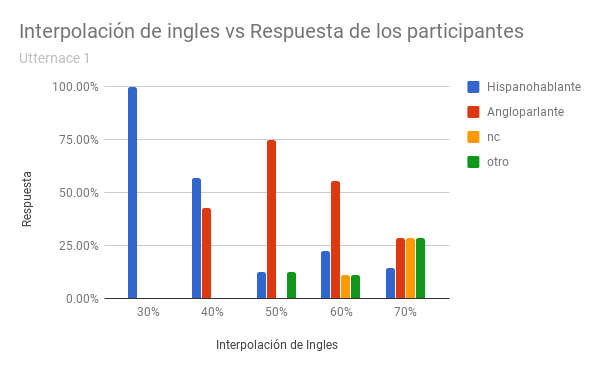
\includegraphics[width=.5\textwidth]{imagenes/nacionalidades/1.png}&
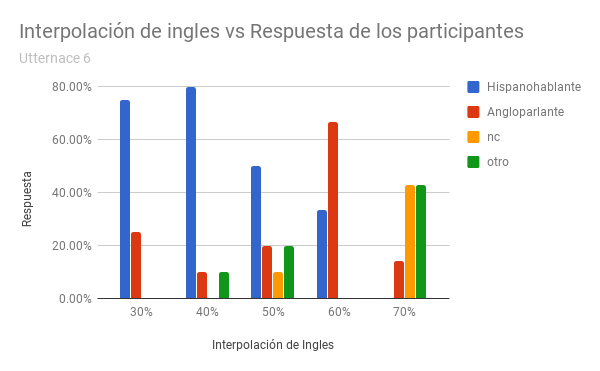
\includegraphics[width=.5\textwidth]{imagenes/nacionalidades/6.png}
\end{array}$
\end{center}
\caption{Oración 1 y 6}
\label{unoSeis}
\end{figure}

\begin{figure}
\begin{center}$
\begin{array}{lll}
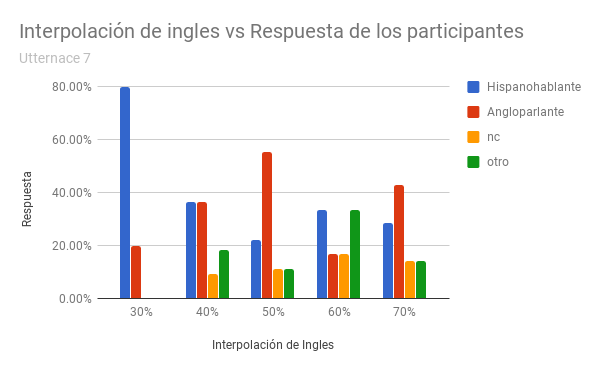
\includegraphics[width=.5\textwidth]{imagenes/nacionalidades/7.png}&
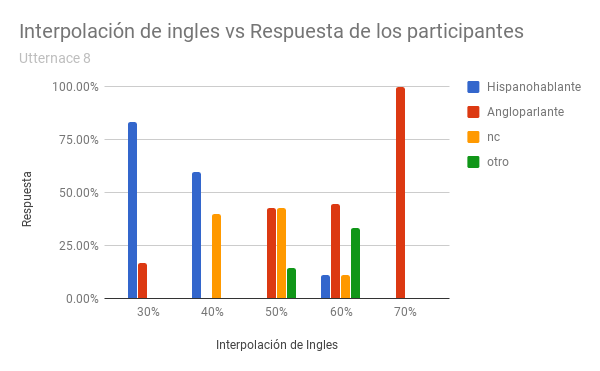
\includegraphics[width=.5\textwidth]{imagenes/nacionalidades/8.png}
\end{array}$
\end{center}
\caption{Oración 7 y 8}
\label{sieteOcho}
\end{figure}

Hasta ahora analizamos los dos ejes de nuestra hipótesis por separado (por un lado, inteligibilidad, por otro, nacionalidad atribuida a la voz). En el ultimo apartado de la investigación buscaremos sacar conclusiones al componer ambos ejes en un mismo análisis.

\section{Resultados Generales de la experimentación}

Por último presentamos la distancia de Levenshtein superpuesto con la probabilidad de un participante de reconocer la voz como un hablante anglosajón.


\begin{figure}
\begin{center}$
\begin{array}{lll}
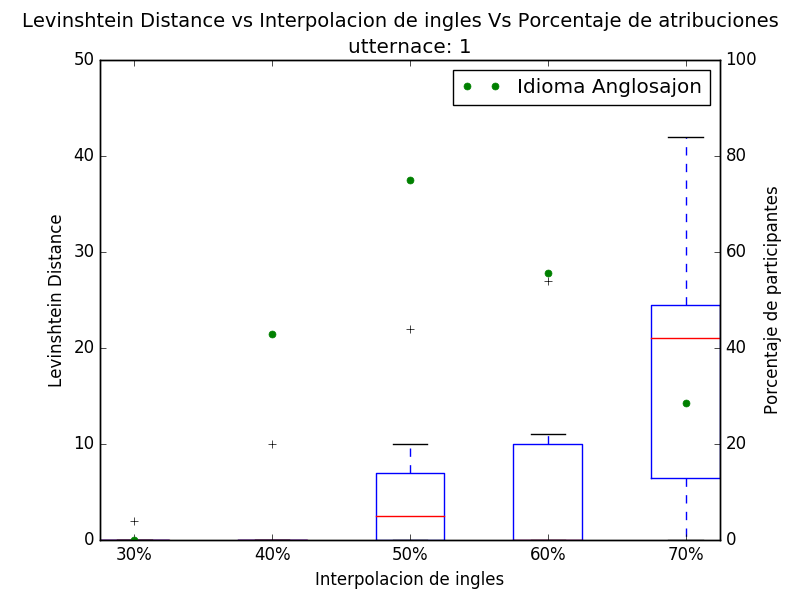
\includegraphics[width=.5\textwidth]{imagenes/nacVsPlot/1.png}&
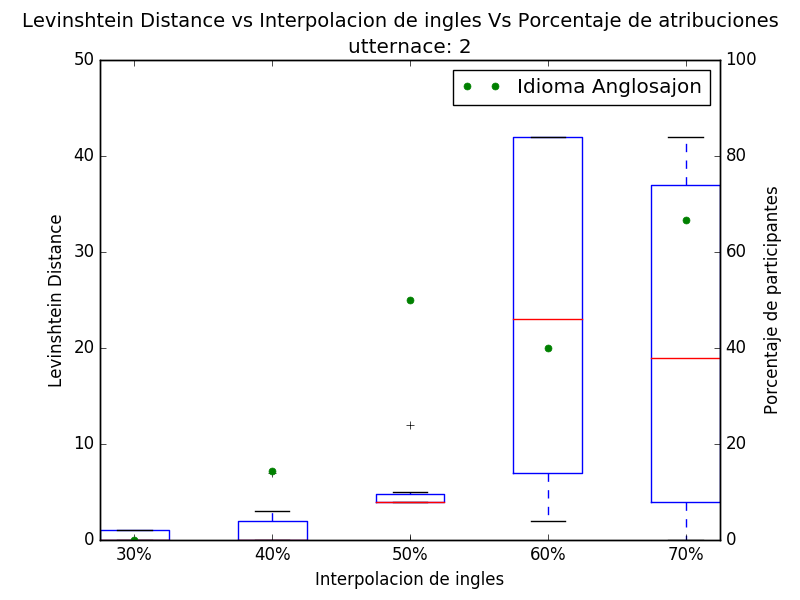
\includegraphics[width=.5\textwidth]{imagenes/nacVsPlot/2.png}
\end{array}$
\end{center}
\caption{Oración 1 y 2}
\label{pics:blablabla}
\end{figure}


Volviendo a la hipótesis original, podemos ver que esta técnica permite generar una voz que pueda ser identificada como un extranjero hablando ingles, con un grado de efectividad que varía desde el $60\%$ hasta el $100\%$ dependiendo de la oración elegido y el grado de interpolación.


\begin{figure}
\begin{center}$
\begin{array}{lll}
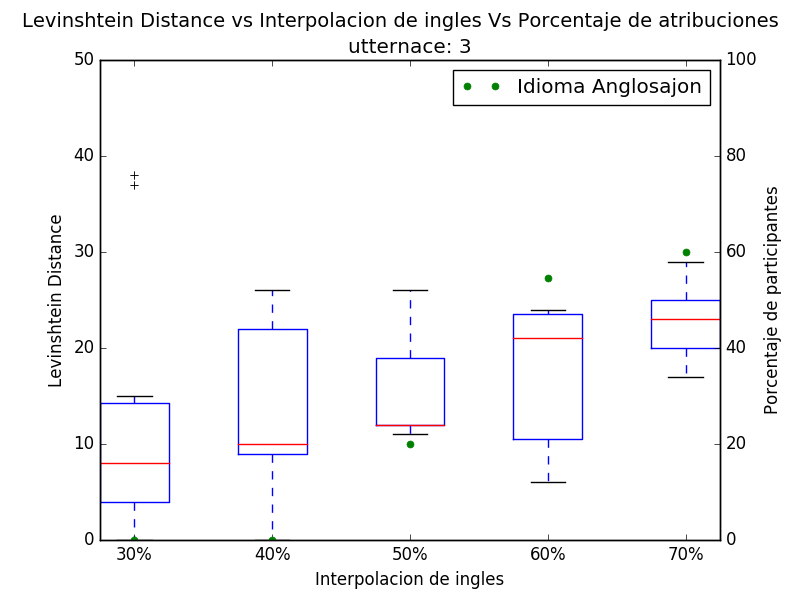
\includegraphics[width=.5\textwidth]{imagenes/nacVsPlot/3.png}&
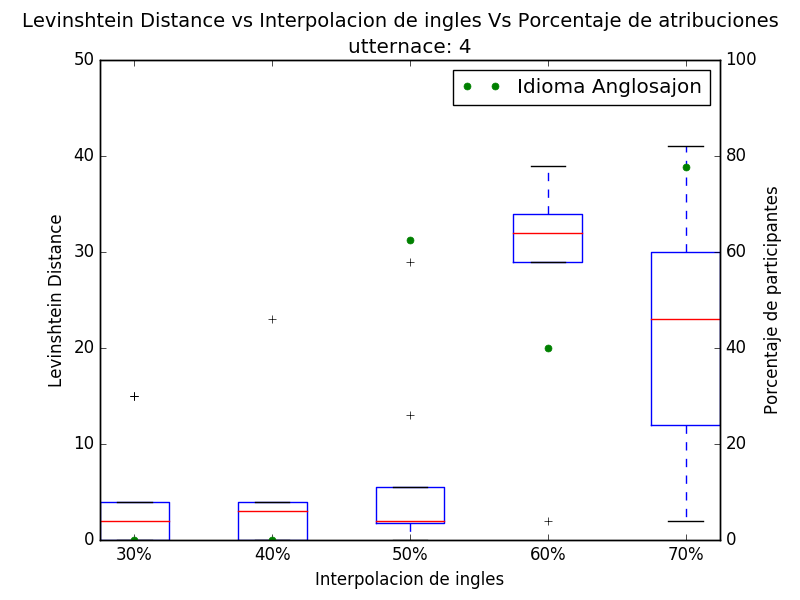
\includegraphics[width=.5\textwidth]{imagenes/nacVsPlot/4.png}
\end{array}$
\end{center}
\caption{Oración 3 y 4}
\label{pics:blablabla}
\end{figure}


También es interesante observar casos como el que se presenta comparando el oración $10$ y la oración $8$, ambos con $70\%$ de mezcla de ingles, que en cuanto a inteligibilidad se encuentran en extremos opuestos, muestran que aproximadamente un $80\%$ y un $100\%$ de participantes identificaron como nativo anglosajón. Esto nos da a pensar que la inteligibilidad de una oración y su probabilidad de ser identificado como un hablante ingles son variables independientes y que este ultimo factor este mas ligado a otros factores como la sonoridad de ciertos fonemas o la prosodia general de la voz. 


Este no es un caso aislado, véase que lo mismo sucede con la oración $4$ y $6$ con $60\%$ de mezcla de ingles, si bien las inteligibilidades están en extremos opuestos, sus probabilidades de ser identificados como hablantes extranjeros difieren en menos del $20\%$.

\begin{figure}
\begin{center}$
\begin{array}{lll}
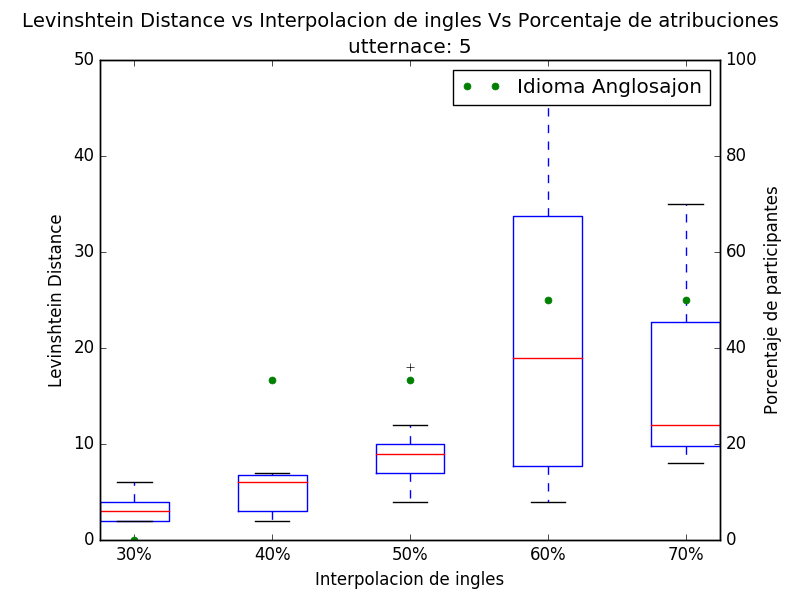
\includegraphics[width=.5\textwidth]{imagenes/nacVsPlot/5.png}&
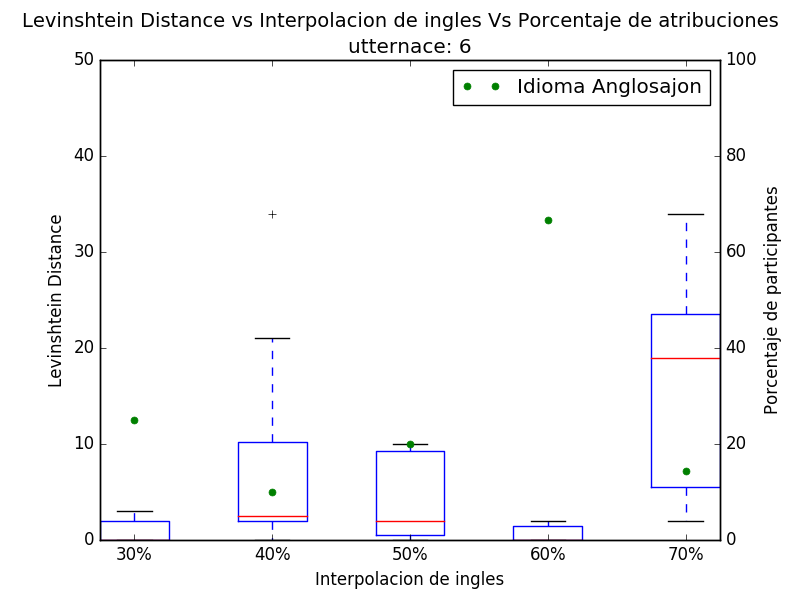
\includegraphics[width=.5\textwidth]{imagenes/nacVsPlot/6.png}
\end{array}$
\end{center}
\caption{Oración 5 y 6}
\label{pics:blablabla}
\end{figure}

\begin{figure}
\begin{center}$
\begin{array}{lll}
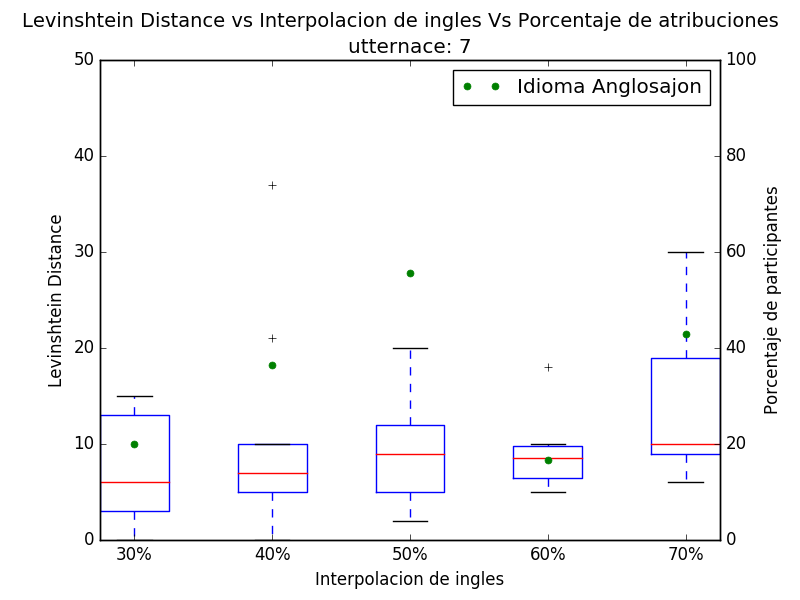
\includegraphics[width=.5\textwidth]{imagenes/nacVsPlot/7.png}&
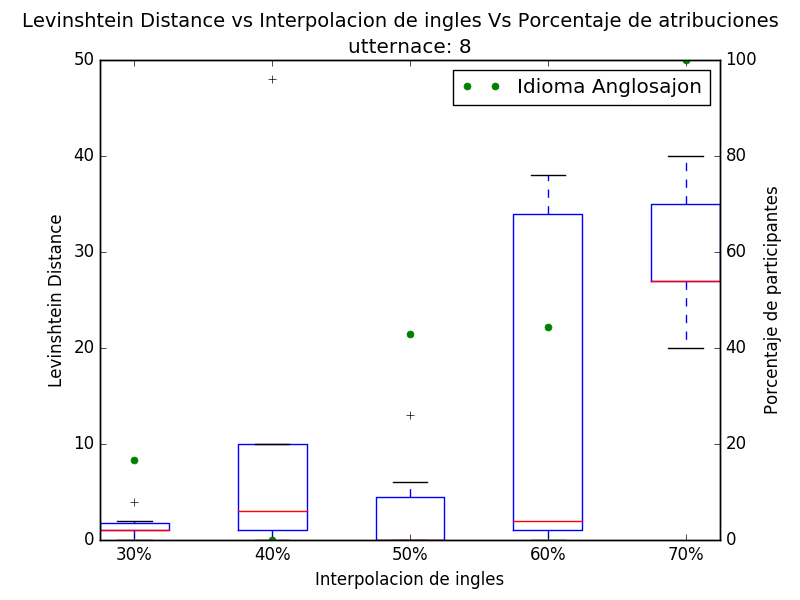
\includegraphics[width=.5\textwidth]{imagenes/nacVsPlot/8.png}
\end{array}$
\end{center}
\caption{Oración 7 y 8}
\label{pics:blablabla}
\end{figure}

\begin{figure}
\begin{center}$
\begin{array}{lll}
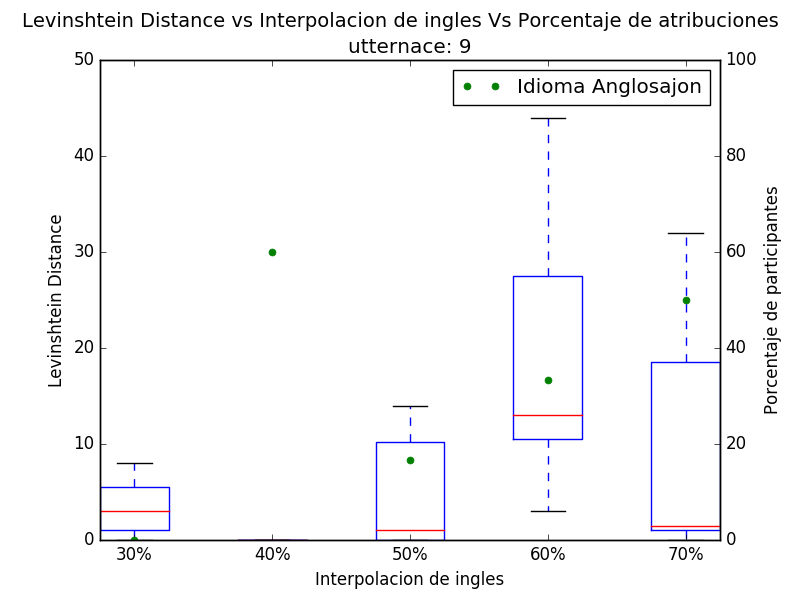
\includegraphics[width=.5\textwidth]{imagenes/nacVsPlot/9.png}&
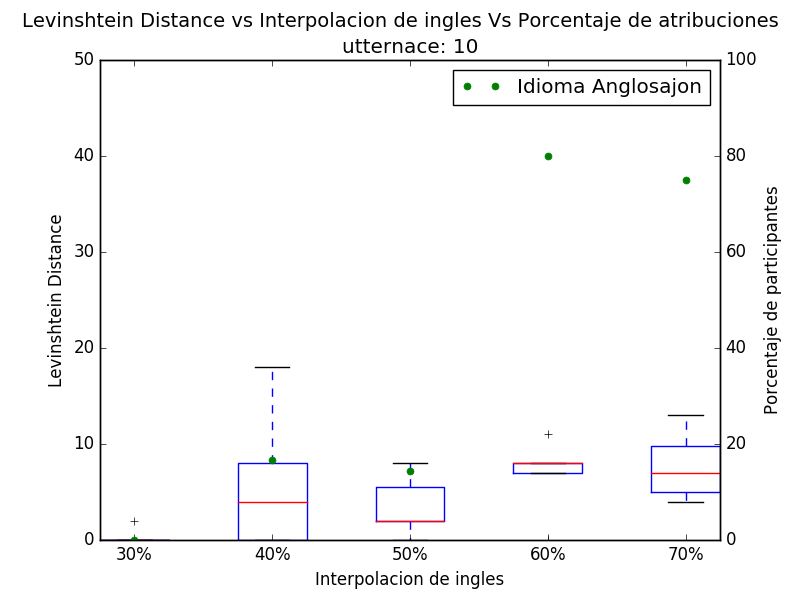
\includegraphics[width=.5\textwidth]{imagenes/nacVsPlot/10.png}
\end{array}$
\end{center}
\caption{Oración 9 y 10}
\label{pics:blablabla}
\end{figure}


\pagebreak

%Final
\section{Trabajo Futuro}

Como fue discutido en la sección de experimentación, una interpolación general puede producir que ciertos fonemas se alejen demasiado del fonema real del castellano, disminuyendo la inteligibilidad de la voz sintetizada. Un posible camino a seguir es realizar una interpolación controlada que permita regular cada fonema por separado. Para fonemas que puedan resultar problematicos como el caso de la /r bibrante el grado de interpolación podría dejarse mas cercano al castellano, mientras que para fonemas con comportamientos mas similares el grado de interpolación podría llevarse mas cerca del modelo ingles.

%expandir
\pagebreak
\section{Apendice}

\section{Transcripciones ingresadas por los participantes} \label{transcripcionesParticipantes}

\noindent Oraciones originales:
\begin{multicols}{2}
\let\mcnewpage=\newpage
\makeatletter
\renewcommand\newpage{%
    \if@firstcolumn
        \hrule width\linewidth height0pt
        \columnbreak
    \else
        \mcnewpage
    \fi
}
\makeatother
\tiny
\centering
\begin{supertabular}{|c|c|}
\hline
#Oración& Transcripción\\
\hline
1&Mi montaña aguileña recorrió la esquina\\
\hline
2&Aquel fuerte vidrio prefirió aquel botón\\
\hline
3&Este enjoyado juez comprará nuestro corchete\\
\hline
4&Tu estrecho posavasos gritó la fechoría\\
\hline
5&Nuestro nublado tigre concluyó a este chupetín\\
\hline
6&Su profundo riñón apoyó a Julio\\
\hline
7&El frío churrasco oyó lo de Polonia\\
\hline
8&Las acongojadas cotorras sonrieron a mi círculo\\
\hline
9&Ese gruñón perro prometió a esos cuñados\\
\hline
10&El nudillo argentino perdió su vaso\\
\hline
\end{supertabular}
\end{multicols}

\noindent Transcripciones: Oración, Mezcla de ingles, Origen, Transcripción

\begin{multicols}{2}
\let\mcnewpage=\newpage
\makeatletter
\renewcommand\newpage{%
    \if@firstcolumn
        \hrule width\linewidth height0pt
        \columnbreak
    \else
        \mcnewpage
    \fi
}
\makeatother
\tiny
\centering
\begin{supertabular}{|p{0.1cm}|p{0.1cm}|p{2cm}|p{3.7cm}|}
\hline
1&30&	Argentina&	Mi montaña aguileña recorrió la esquina	\\
\hline
1&30&	Argentino&	Mi montaña aguileña recorrio la esquina	\\
\hline
1&30&	española&	mi montaña aguileña recorrió la esquina	\\
\hline
1&30&	Norte argentino&	Mi montaña aguileña recorrió la esquina	\\
\hline
1&30&	argentina&	mi montania aguilenia recorrió la esquina	\\
\hline
1&30&	Latino&	Mi montaña aguileña recorrió la esquina	\\
\hline
1&40&	Español&	Mi montaña aguileña recorrió la esquina	\\
\hline
1&40&	Ingles&	MI montaña aguileña recorrió la esquina	\\
\hline
1&40&	Uruguay&	Mi montaña recorrió la esquina	\\
\hline
1&40&	Argentina&	mi montaña aguileña recorrió la esquina	\\
\hline
1&40&	centroamerica&	Mi montaña aguileña recorrió la esquina	\\
\hline
1&40&	estadounidense&	mi montaña aguileña recorrio la esquina	\\
\hline
1&40&	EEUU&	Mi montaña aguileña recorrió la esquina	\\
\hline
1&50&	Boliviana&	Mi montaña recorrio la esquina	\\
\hline
1&50&	EEUU hablando español&	mi montaña milenia recorrió la esquina	\\
\hline
1&50&	Inglés&	Mi montaña aguileña recorrio la esquina	\\
\hline
1&50&	Japonés&	Recorrio la esquina	\\
\hline
1&50&	norteamericana&	mi montaña aguileña recorrió la esquina	\\
\hline
1&50&	Inglesa&	mi montaña pedigüeña recorrió la esquina	\\
\hline
1&50&	Estadounidense&	mi montaña aguileña recorrio la esquina	\\
\hline
1&50&	Estadounidense&	mi montaña aguileña recorrió la esquina	\\
\hline
1&60&	estadounidense&	Mi montaña aguileña recorrió la esquina	\\
\hline
1&60&	Estados unidos&	Mi montaña aguilenia recorrió la esquina	\\
\hline
1&60&	Irlanda&	Mi montaña aguileña recorrió la esquina.	\\
\hline
1&60&	Norte argentino&	Mi montaña aguileña recorrió la esquina	\\
\hline
1&60&	catellano&	recorriendo la esquiena	\\
\hline
1&60&	EEUU&	mi montaña aguileña recorrió la esquina	\\
\hline
1&60&	No se especifica&	Mi montaña..... recorrió la esquina	\\
\hline
1&60&	eeuu&	mi montaña aguileña recorrió la esquina	\\
\hline
1&60&	frances&	mi montaña recorrió la esquina	\\
\hline
1&70&	Ninguna&	Mi monzonia la cigüeña recorrio la esquina	\\
\hline
1&70&	Italiano&	Corrio a la esquina	\\
\hline
1&70&	Castellano&	Recorrió la esquina	\\
\hline
1&70&	Guam&	Mí montoña aguileña recorrió la esquina	\\
\hline
1&70&	Canadá&	Mi montaña aguileña recorrió la esquina	\\
\hline
1&70&	EEUU&	Mi corrió la esquina	\\
\hline
1&70&	nose&		\\
\hline
2&30&	argentino&	Aquel fuerte vidrio prefirió aquel botón	\\
\hline
2&30&	Ninguna&	Aquel fuerte vidrio prefirio aquel boton	\\
\hline
2&30&	Ninguna&	Aquel fuerte vidrio prefirió aquel botón	\\
\hline
2&30&	Argentino&	aquel fuerte vidrio prefirio aquel boton	\\
\hline
2&30&	Chile&	aquel fuerte vidrio prefirió aquel botón	\\
\hline
2&30&	Argentina&	aquel fuerte vidrio prefirió aquel botón	\\
\hline
2&40&	Espa;ol&	Aquel fuerte vidrio prefirio aquel boton	\\
\hline
2&40&	Ingles&	Aquie fuerte vidrio prefirio aquel boton	\\
\hline
2&40&	Argentino&	Aquel fuerte vidrio prefirio aquel boton	\\
\hline
2&40&	Norte argentino&	Aquel fuerte vidrio prefirió aquel botón	\\
\hline
2&40&	centroamericana&	aquel fuerte vidrio prefirió aquel boton	\\
\hline
2&40&	argentina&	aquel fuerte vidrio percibió al boton	\\
\hline
2&40&	Gallega&	Aquel fuerte vidrio prefirió aquel botón.	\\
\hline
2&50&	Inglesa&	Aqueo fuerte vidrio perforo aquel boton	\\
\hline
2&50&	paraguay&	aquel vidrio presiono aquel boton	\\
\hline
2&50&	francés&	aquél fuerte vidrio prefirió aquél botón	\\
\hline
2&50&	Estados Unidos&	aquel fuerte vidrio percibió aquel botón	\\
\hline
2&50&	EEUU&	Aquel fuerte vidrio prefirió aquel botón	\\
\hline
2&50&	Mexicano&	Aquel fuerte vidrio percibió aquel botón	\\
\hline
2&60&	inglesa&	aquel fuerte vidrio presidió aquel botón	\\
\hline
2&60&	Santo Domingo&	Aquel Fuel de vidrio prefiere aquel boton	\\
\hline
2&60&	paraguay&	te voy a pegar un palazo en la nuca y romperte el orto	\\
\hline
2&60&	estadounidense&	prefirió el botón	\\
\hline
2&60&	China&		\\
\hline
2&70&	Ingles&		\\
\hline
2&70&	Estados unidos&	Preferido aquel boton	\\
\hline
2&70&	inglesa&	aquel blablaba prefirio aquel boton	\\
\hline
2&70&	No se especifica&	Aquel fuerte vidrio prefirió aquel botón	\\
\hline
2&70&	Ninguna, es un robot.&		\\
\hline
2&70&	EEUU&	Aquel fuerte vidrio prefirió aquel boton	\\
\hline
3&30&	Argentino&	Este enjollado puede comparar nuestro cochete	\\
\hline
3&30&	Argentina&	Este enfueyado fue comparado corchete	\\
\hline
3&30&	Español&	Corchete	\\
\hline
3&30&	Argentino capital federal&	Corchete	\\
\hline
3&30&	Robot&	Este enrollado fue comprado nuestro corchete	\\
\hline
3&30&	española&	este enjoyado juez comprará nuestro corchete	\\
\hline
3&30&	Paraguayo&	este enjoyado fue comprado este corchete	\\
\hline
3&30&	Argentino&	Este enfollado juez comprará nuestro corchete	\\
\hline
3&30&	Español&	Este enfollado fue comprar nuestro corchete	\\
\hline
3&30&	No se especifica&	Este enjoyado juez comprará nuestro corchete	\\
\hline
3&30&	Indefinida&	Este enjoyado fue comprado corchete	\\
\hline
3&40&	La Rioja, Argentina&	Este encollado encontrará nuestro corchete	\\
\hline
3&40&	Ninguna nacionalidad&	Este fue juez corchete	\\
\hline
3&40&	España&	este enfollado comprara nuestro corchete	\\
\hline
3&40&	Española&	este fue nuestro corchete	\\
\hline
3&40&	Español neutro&	este enjoyado juez comprará nuestro corchete	\\
\hline
3&50&	Boliviano&	Este juez comprara nuestro	\\
\hline
3&50&	anglo&	este enrollado corchete	\\
\hline
3&50&	Maracaibo&	Este enconchado puede comprado nuestro cohete	\\
\hline
3&50&	Colombiano/Venezolano&	Este enfollado fue encontrar nuestro corchete	\\
\hline
3&50&	No se&	Este enrollado fue encontrar nuestro coechete	\\
\hline
3&60&	Ninguna&	Este en...fue comprar nuestro corchete	\\
\hline
3&60&	Inglesa&	Este nuestro corchete	\\
\hline
3&60&	gallego&	este enfollado comprara nuestro corchete	\\
\hline
3&60&	Ingles&	Este enfollado juez comprara nuestro corchete	\\
\hline
3&60&	inglés&	compraran nuestro corchete	\\
\hline
3&60&	Español&	Este ??? pues comprará nuestro corchete	\\
\hline
3&60&	estadounidense o inglés&	este ... nuestro corchete	\\
\hline
3&60&	estadounidense&	este fue nuestro corchete	\\
\hline
3&60&	Argentino&	Esté nuestro corchete	\\
\hline
3&60&	americano (EEUU)&	estoy nuestro corchete	\\
\hline
3&60&	Desconocido&	Comprara nuestro corchete	\\
\hline
3&70&	alemania&	este enfollado fuescon cuero nuestro follete	\\
\hline
3&70&	Hablante nativo de inglés& 	este ..... fue ..... en nuestro corchete	\\
\hline
3&70&	estadounidense&	este vuestro corchete	\\
\hline
3&70&	Ruso&	este fue encontrado con nuestro coche	\\
\hline
3&70&	estadounidense&	nuestro corchete	\\
\hline
4&30&	Argentina&	Tu estrecho posa basos grito la fechoria	\\
\hline
4&30&	Argentina&	Tu estrecho posa vasos grito	\\
\hline
4&30&	Cigbord&	Gritemos portavasos gritona fechoria	\\
\hline
4&30&	parece& una voz artificial	Tu estrecho posavasos gritó la fechoría	\\
\hline
4&30&	españa&	tu estrecho posavasos gritó la fechoría	\\
\hline
4&30&	Española&	Tu estrecho posavasos gritó la fechoría	\\
\hline
4&30&	no sé&	su estrecho posavasos gritó en la fechoría	\\
\hline
4&30&	Española&	Tu estrecho posa vasos gritó la fechoría	\\
\hline
4&30&	centroamericano&	fui estrecho posavasos grito la fechoría	\\
\hline
4&30&	español neutro&	tu estrecho posavasos gritó la fechoría	\\
\hline
4&40&	español de españa&	tu estrecho posavasos grito la fechoria	\\
\hline
4&40&	España&	Tu estrecho posavasos gritó la fechoría	\\
\hline
4&40&	Español&	Si estrecho posa vaso	\\
\hline
4&40&	España&	tu estrecho posavasos gritó la fechoría	\\
\hline
4&40&	Argentina&	Tu estrecho posa vasos grito la fechoriay	\\
\hline
4&50&	anglo&	tu estrecho posa vasos grito la fechoria	\\
\hline
4&50&	Ingles&	Su estrecho posavazos gritó la fechoría	\\
\hline
4&50&	Ingles&	Su estrecho posavazos gritó la fechoría	\\
\hline
4&50&	italiano&	la fechoria	\\
\hline
4&50&	inglés&	su estrecho posavasos gritó la fechoria	\\
\hline
4&50&	estadounidense&	tu estrecho posavasos gritó la fechoría	\\
\hline
4&50&	Cuba&	tu estrecho posavasos, grito la fechoría	\\
\hline
4&50&	Española&	Su estrecho posavaso fechoría	\\
\hline
4&60&	Francés&	Frechoia	\\
\hline
4&60&	chino mandarin	&chu ...	\\
\hline
4&60&	Colombia&	Tu estrecho posavasos grito la fechoria	\\
\hline
4&60&	Eeuu&	Posavasos	\\
\hline
4&60&	estaunidense&	... la fechoría	\\
\hline
4&70&	estadounidense&	la fechoria	\\
\hline
4&70&	Estados& Unidos	tu estrecho posavasos	\\
\hline
4&70&	no lo pude determinar, osea es una maquina&	las fechorias (al final de todo)	\\
\hline
4&70&	Australia&	You	\\
\hline
4&70&	ns/nc&	ns/nc	\\
\hline
4&70&	inglesa&	su estrecho posavasos gritó  la fechoría	\\
\hline
4&70&	Hablante nativo de inglés&	tu estrecho posavasos .. la fechoría	\\
\hline
4&70&	americana (EEUU)&	tu estrecho portavasos fechoria	\\
\hline
4&70&	estadounidense&	vasos la fechoría	\\
\hline
5&30&	Castellano&	Nuestro nublado tigre concluyo a este chupetin	\\
\hline
5&30&	Española&	Nuestro nublado tigre concluyó a esta chupetin	\\
\hline
5&30&	Sin nacionalidad&	Nuestro nublado tigre concluyó a este chupetin	\\
\hline
5&30&	argentina&	nuestro nublado tigre concluyó a este chupetín	\\
\hline
5&30&	Neutro&	Nuestro nublado tigre concluyó a este chupetin	\\
\hline
5&30&	argentina&	nuestro nublado tigre concluyó a nuestro chupetín	\\
\hline
5&40&	Argentina&	Nuestro nublado día concluyó a este chupetin	\\
\hline
5&40&	Alemana&	Nuestro nublado vive concluyó este chupetin	\\
\hline
5&40&	Inglesa&	nuestro nublado y reconcluyó a este chupetín	\\
\hline
5&40&	EEUU&	nuestro nublado tigre concluyo este chupetin	\\
\hline
5&40&	Argentino&	nuestro nublado tigre concluyó a este chupetín	\\
\hline
5&40&	español&	Nuestro nublado tigre concluyó a este chupetín	\\
\hline
5&50&	ciudad de buenos aires&	nuestro nublado concluyo este chupetin	\\
\hline
5&50&	Google&	Nuestro nublado vive concluyo a este chupetín	\\
\hline
5&50&	estadounidense&	nuestro nublado tigre concluyó este chupetín	\\
\hline
5&50&	Robot del traductor de Google&	Nuestro hermano encontró este chupetín (?)	\\
\hline
5&50&	inglés&	Nuestro nublado día concluyó este chupetín	\\
\hline
5&50&	estaunidense&	nuestro nublado tigre concluyó este chupetín	\\
\hline
5&50&	Robot&.	Nuestro nublado concluyó este chupetín	\\
\hline
5&50&	español& neutro	nuestro nublado ... concluyó a este chupetín	\\
\hline
5&50&	Argentina&	Nuestro nublado y reconstruyó a este chupetín	\\
\hline
5&60&	Español&		\\
\hline
5&60&	Chile&	nuestro ... chupetin	\\
\hline
5&60&	español&	este chupetin	\\
\hline
5&60&	Estados Unidos&	nuestro nublado concluyó este chupetín	\\
\hline
5&60&	Eeuu&	Nuestro nublado y re concluyó este chupetin	\\
\hline
5&60&	Español& neutro	Nuestro ... este chupetin	\\
\hline
5&60&	Inglés/Estado Unidense&	Nuestro nublado tigre concluyó este chupetin	\\
\hline
5&60&	estadounidense o inglés&	nuestro nublado y reconcluyó este chupetín	\\
\hline
5&70&	polaco&	nuestro reconstruye este chupetìn	\\
\hline
5&70&	Portugués&	Nuestro pequin	\\
\hline
5&70&	Estadounidense&	Nuestro nublado construyó este chupetin	\\
\hline
5&70&	Estados unidos&	Nuestro nublado libre construyó este chupetín	\\
\hline
5&70&	Estadounidense&	nuestro ... este chupetín	\\
\hline
5&70&	Panama&	nuestro anublado reconcluyo este chupetin	\\
\hline
5&70&	Argentina&	Nuestro nublado concluyó a este chupetín	\\
\hline
5&70&	estadounidense&	nuestro nublado concluyó este chupetín	\\
\hline
6&30&	Español&	Su profundo riñón apoyo a Julio	\\
\hline
6&30&	Argentino&	Su profundo riñón apoyó a Julio	\\
\hline
6&30&	Argentina&	su profundo riñon apoyo a Julio	\\
\hline
6&30&	estados unidos&	su profundo riñón apoyó a Julio	\\
\hline
6&30&	argentina&	su profundo riñón apoyó a julio	\\
\hline
6&30&	Española&	Su profundo riñón apoyó a a Julio	\\
\hline
6&30&	Argentino&	Su profundo riñón apoyó a Julio	\\
\hline
6&30&	Ingles&	Su profundo riñón apoyo a Julio	\\
\hline
6&40&	Colombiano&	Su profundo riñón apoyo a julio	\\
\hline
6&40&	frances&	nada	\\
\hline
6&40&	argentina&	si lo profundo julio	\\
\hline
6&40&	Paraguayo&	Profundo riñon julio	\\
\hline
6&40&	Argentino&	Su profundo riñón apoyo a julio	\\
\hline
6&40&	Español neutro/Rioplatense& Su profundo riñon apoyo a Julio	\\
\hline
6&40&	EEUU&	su profundo riñon apoyo junio	\\
\hline
6&40&	Argentina&	su profundo riñon apoyó a julio	\\
\hline
6&40&	Argentino&	Su profundo riñón apoyo a julio	\\
\hline
6&40&	Argentina&	Su profundo riñón apoyó a Julio	\\
\hline
6&50&	polaco&	si profundo donde apoyo a julio	\\
\hline
6&50&	Castellano&	Su profundo riñon apoyo a julio	\\
\hline
6&50&	Argentino&	Su profundo riñon julio	\\
\hline
6&50&	Francia&	su profundo riñor apoyo a	\\
\hline
6&50&	no es hispano parlante& su profundo riñon de apoyo julio	\\
\hline
6&50&	Peru&	su profundo riñon apoyo a Julio	\\
\hline
6&50&	español centroamérica& 	su profundo riñon apoyó a Julio	\\
\hline
6&50&	Inglesa&	su profundo riñón apoyó a Julio	\\
\hline
6&50&	Argentina&	Su profundo riñón apoyo a julio	\\
\hline
6&50&	estadounidense&	Su profundo riñón apoyó a julio	\\
\hline
6&60&	estados unidos&	su profundo riñon apoyo a julio	\\
\hline
6&60&	Estadounidense&	su profundo riñón apoyó a Julio	\\
\hline
6&60&	Estadounidense&	Su profundo riñón apoya a julio	\\
\hline
6&60&	Argentina&	Su profundo riñón apoyó a Julio	\\
\hline
6&60&	cordobés&	su profundo riñón apoyó a julio	\\
\hline
6&60&	estadounidense&	su profundo riñón apoyó a julio	\\
\hline
6&70&	Google&	Su profundo riñón apoyó a su higado	\\
\hline
6&70&	Rusia&		\\
\hline
6&70&	google translate&	supra india fidileia	\\
\hline
6&70&	estadounidense&	su profundo riñón apoyo afilio	\\
\hline
6&70&	Robot&	Su profundo	\\
\hline
6&70&	Japones&	Si profundo neanea nou	\\
\hline
6&70&	china&	su profundo riñon apoyó a julio	\\
\hline
7&30&	Estadounidense&	el frío churrasco yo lo de Polonia	\\
\hline
7&30&	Argentina&	El frío churrasco oyó lo de Polonia	\\
\hline
7&30&	Colombia&	el frio churrasco de colombia	\\
\hline
7&30&	argentina&	el frío churrasco lleno de polonia	\\
\hline
7&30&	chile&	el frio solo de polonia	\\
\hline
7&40&	Español&	Churrasco, Polonia	\\
\hline
7&40&	estados unidos&el frio churrasco de polonia	\\
\hline
7&40&	español&		\\
\hline
7&40&	Estadounidense&	Enfrío churrasco "goyono" de Polonia	\\
\hline
7&40&	Española&	el frio churrasco frio de Polonia	\\
\hline
7&40&	Español&	Enfrió churrasco en solo de polonia	\\
\hline
7&40&	ni idea'); &	el frio churrasco oyó lo de Polonia	\\
\hline
7&40&	Inglesa&	EL frío churrasco ozono de Polonia	\\
\hline
7&40&	estadounidense&	el frío churrasco oyó lo de Polonia	\\
\hline
7&40&	Neerlandes&	Enfrio churrasco yo no de polonia	\\
\hline
7&40&	Japones&	Enfrió churrasco frío de polonia	\\
\hline
7&50&	Español&	Enfrio churrascos anchos de Polonia	\\
\hline
7&50&	Inglesa&	El frío churrasco yo como de colombia	\\
\hline
7&50&	Inglés o Irlandés&	churrasco Polonia	\\
\hline
7&50&	computadora&	en frio churrasco yo no de polonia	\\
\hline
7&50&	EEUU&	Enfrío churrasco lleno de poloña.	\\
\hline
7&50&	Estados unidos&	enfrío churrasco oyó lo de polonia	\\
\hline
7&50&	Brasiltino&	Enfrio churrasco o jogo de Polonia	\\
\hline
7&50&	Argentina&	el frio churrasco ollolo de polonia	\\
\hline
7&50&	Ingles&	Enfrió churrasco de polonia	\\
\hline
7&60&	Castellano&	Frio churrasco lleno de colonia	\\
\hline
7&60&	Argentino&	El frío churrasco de Polonia	\\
\hline
7&60&	Polonia&	El frío churrasco	\\
\hline
7&60&	Francia&	el frio churrasco de polonia	\\
\hline
7&60&	Estados Unidos (google translate...)&	el frio churrasco llego de polonia	\\
\hline
7&60&	ninguna&	el frío churrasco moncholo de polonia	\\
\hline
7&70&	Google&	El frio churrasco de polonia	\\
\hline
7&70&	inglés&	polonia	\\
\hline
7&70&	eeuu&	el frio churrasco de polonia	\\
\hline
7&70&	EEUU&	El frio churrasco de polonia	\\
\hline
7&70&	Argentina&	El frío churrasco cayo de Polonia	\\
\hline
7&70&	Quichua&	Churrasco	\\
\hline
7&70&	Argwntino&	El frió churrasco lleno de  Colonia	\\
\hline
8&30&	España (Sur)&	Las acongojadas cotorras sonrieron a mi círculo.	\\
\hline
8&30&	EEUU&	Las acongojadas cotorras sonrieron a mi círculo.	\\
\hline
8&30&	argentina&	Lss acongojadas cotorras sonrieron a circulo	\\
\hline
8&30&	Argentina&	Las acongojadas cotorras sonrieron a mi círculo	\\
\hline
8&30&	Latino&	Las acongojadas cotorras sonrieron a mi circulo	\\
\hline
8&30&	Español&	Las acongojadas cotorras corrieron a mi circulo	\\
\hline
8&40&	Español&	Las acontojadas culturas Sonrieron en semicirculo	\\
\hline
8&40&	Argentino&	Las acombojadas cotorras sonrieron a mi círculo	\\
\hline
8&40&	Google&	Las acongojadas cotorras sonrieron a mi circulo	\\
\hline
8&40&	Latino&	Las acongojadas cotorras sonrieron a mi círculo	\\
\hline
8&40&	asd&	asd	\\
\hline
8&50&	Francia&	las  cotorras sonrieron en mi circulo	\\
\hline
8&50&	Nose&	Las acongojadas cotorras sonrieron a mi circulo	\\
\hline
8&50&	Ninguno&	Las acongojadas cotorras sonrieron a mi círculo	\\
\hline
8&50&	Estadounidense&	Las acongojadas cotorras vinieron a mi círculo	\\
\hline
8&50&	Ingles/estadounidense&	Las acongojadas cotorras sonrieron a mi circulo	\\
\hline
8&50&	ninguna&	las acongojadas cotorras sonrieron a mi círculo	\\
\hline
8&50&	estadounidense&	las aconogojadas cortorras se unieron a mi círculo	\\
\hline
8&60&	Español&	De mi circulo	\\
\hline
8&60&	Estadounidense&	En mi circulo	\\
\hline
8&60&	Estadounidense&	Las acongojadas cotorras sonrieron a mi círculo	\\
\hline
8&60&	Inglesa&	Mi círculo	\\
\hline
8&60&	Rusa&	Las acongojadas cotorras sonrieron a mi círculo	\\
\hline
8&60&	EEUU&	las acongojadas cotorras sonrieron en mi circulo	\\
\hline
8&60&	No hispanohablante&	las acongoyadas cotorras sonrieron a mi circulo	\\
\hline
8&60&	rusa&	las acongojadas cotorras sonrieron en mi circulo	\\
\hline
8&60&	Francesa&	Las acongojadas cotorras sonrieron en mi círculo	\\
\hline
8&70&	estadounidense&	círculo	\\
\hline
8&70&	estadounidense&	some hemicírculo	\\
\hline
8&70&	inglés&	sonrieron en mi circulo	\\
\hline
8&70&	Estadounidense&	... sonrieron en mi círculo	\\
\hline
8&70&	eeuu&	plaza sombreada con sombrero sonrieron en mi círculo	\\
\hline
9&30&	Español&	Ese gruñon perro prometio a esos cuñados	\\
\hline
9&30&	Argentina&	Ese gruñón Prometió a sus cuñados	\\
\hline
9&30&	Paraguayo&	Ese gruñon me lo prometio a esos cuñados	\\
\hline
9&30&	español&	ese gruñon se lo prometio a esos cuñados	\\
\hline
9&30&	Argentino&	el se reunión pero prometió a esos cuñados	\\
\hline
9&30&	Rusa&	Ese gruñón perro prometió a esos cuñados	\\
\hline
9&30&	Argentina&	Ese gruñon perro prometio esos cuñados	\\
\hline
9&40&	Francia o Suiza&	Ese gruñón perro prometió a esos cuñados.	\\
\hline
9&40&	estadounidense&	Ese gruñón perro prometió a esos cuñados	\\
\hline
9&40&	Chilena&	Ese gruñón perro prometió a esos cuñados	\\
\hline
9&40&	estadounidense&	ese gruñón perro prometió a esos cuñados	\\
\hline
9&40&	eeuu&	ese grunion perro prometió a esos cuñados	\\
\hline
9&50&	Google&	Ese gruñon perro prometio a esos cuñados	\\
\hline
9&50&	puerto rico&	ese gruñón perro prometió esos cuñados	\\
\hline
9&50&	Estados unidos&	pero prometió a esos cuñados	\\
\hline
9&50&	es un robot&	el segundo *** prometio a esos cuñados	\\
\hline
9&50&	ucrania&	ese gruñon perro prometió a esos cuñados	\\
\hline
9&50&	Mexico&	ese gruñón perro prometió a esos cuñados	\\
\hline
9&60&	Sueco&	Ese gruñon prometio esos cuñados	\\
\hline
9&60&	españa&	Ese gruñón peón prometió a esos cuñados	\\
\hline
9&60&	a&	esas cuñadas	\\
\hline
9&60&	H&	J	\\
\hline
9&60&	Ingles&	Esa reunion prometiò a esos cuñados	\\
\hline
9&60&	Anglo& parlante	Ese gruñón perro a esos cuñados	\\
\hline
9&70&	Ingles&	Its a pair of promises	\\
\hline
9&70&	Estadounidense&	Ese gruñón pero prometió a esos cuñados	\\
\hline
9&70&	Estadounidense&	Ese gruñón pero prometió a esos cuñados	\\
\hline
9&70&	...&	ese gruñón perro prometio a esos cuñados	\\
\hline
9&70&	Aleman&	ese gruñon perro prometió a esas cuñadas	\\
\hline
9&70&	Ruso&	Rsts reunion que prometió a sus...	\\
\hline
10&30&	Español&	El nudillo argentino perdio su vaso	\\
\hline
10&30&	Argentino&	El nudillo argentino perdio su vaso	\\
\hline
10&30&	Argentina&	El novillo argentino perdió su vaso	\\
\hline
10&30&	Español&	El nudillo argentino perdio su vaso	\\
\hline
10&30&	argentina&	el nudillo argentino perdió su vaso	\\
\hline
10&30&	Argentina&	el nudillo argentino perdió su vaso	\\
\hline
10&40&	-&	El argentino perdió su vaso	\\
\hline
10&40&	...&	el nudillo argentino perdió su vaso	\\
\hline
10&40&	argentina&	el nudillo argentino perdio su vaso	\\
\hline
10&40&	argentino&	el argentino perdió su vaso	\\
\hline
10&40&	ingles&	el nudillo argentino perdió su vaso	\\
\hline
10&40&	Argentino&	El....perdió su vaso	\\
\hline
10&50&	Español&	El nudillo argentino perdió su vaso	\\
\hline
10&50&	Mexico&	el novillo argentino perdió su vaso	\\
\hline
10&50&	argentina&	el novillo argentino perdió su vaso	\\
\hline
10&50&	español&	el brillo argentino perdio su vaso	\\
\hline
10&50&	No se especifica&	Individuo argentino perdió su vaso	\\
\hline
10&50&	Ingles&	El novillo argentino perdió su vaso	\\
\hline
10&50&	.?&	El argentino perdió su vaso	\\
\hline
10&60&	Estados unidos&	El Argentino perdio su vaso	\\
\hline
10&60&	estadounidense&	El ... argentino perdió su vaso	\\
\hline
10&60&	robot&	el nudillo argentino perdio su vaso	\\
\hline
10&60&	EEUU&	argentino perdió su vaso	\\
\hline
10&60&	amerciano (EEUU)&	un chico argentino perdió su vaso	\\
\hline
10&70&	estadounidense&	El chico argentino perdió su vaso	\\
\hline
10&70&	estadounidense&	el nuevo dj argentino perdió su vaso	\\
\hline
10&70&	Taiwán&	El ... argentino perdió su vaso.	\\
\hline
10&70&	Estadounidense&	El nuevo argentino perdio su vaso	\\
\hline
10&70&	Computadorlandia&	El indígena argentino perdió su vaso	\\
\hline
10&70&	estadounidense&	argentino perdió su vaso	\\
\hline
10&70&	estadounidense&	el susuño argentino perdió su vaso	\\
\hline
10&70&	Estados Unidos&	... argentino perdio su casa	\\
\hline
\end{supertabular}
\end{multicols}
\section{Referencias}
\begin{itemize}
\item $[1]$Statistical Parametric Speech Synthesis Based on Speaker and Language Factorization, Heiga Zen, Member, IEEE, Norbert Braunschweiler, Sabine Buchholz, Mark J. F. Gales, Fellow, IEEE, Kate Knill, Member, IEEE, Sacha Krstulovic, and Javier Latorre, Member, IEEE
\item $[2]$Speaker Similarity Evaluation Of Foreign-accented Speech Synthesis Using Hmm-based Speaker Adaptation, Mirjam Wester, Reima Karhila
\item $[3]$Simultaneous Modeling of phonetic and prosodic parameters, and characteristic conversion for hmm-based text-to-speech systems, takayoshi yoshimura
\end{itemize}
\backmatter
%\bibliography{tesis}
\end{document}
